\documentclass[12pt,a4paper,oneside]{book}

\usepackage[T1]{fontenc}
\usepackage[utf8]{inputenc}
%\usepackage[english]{babel}
\usepackage{lmodern}
\usepackage{amsmath,latexsym,amsthm,amsfonts,epsfig}
\usepackage{graphicx}
\usepackage{svg}
\usepackage{tabularx}
\usepackage{pdflscape}
\usepackage{lipsum}
\usepackage[linesnumbered,ruled,vlined]{algorithm2e}
\usepackage{color}
\usepackage{afterpage}
\usepackage{rotating}
\usepackage[left=3.5cm, right=2.5cm]{geometry} 
\usepackage{graphicx}
\usepackage{listings}% listing kodu
\usepackage{dcolumn}
\usepackage{fancybox}
\usepackage{float}
\usepackage{multirow}
\usepackage{longtable}
\usepackage{url}
\usepackage{enumerate}
\usepackage[titletoc]{appendix}
\usepackage{fancyhdr}
\pagestyle{fancy}
\graphicspath{{./graphics/}}
\fancyhf{}
% numery stron: lewa do lewego (marginesu), prawa do prawego 
\fancyhead[LE,RO]{\textbf{\thepage}} 
% prawa pagina: zawartość \rightmark do lewego, wewnętrznego (marginesu) 
\fancyhead[LO]{\small\sffamily \nouppercase{\rightmark}}
% lewa pagina: zawartość \leftmark do prawego, wewnętrznego (marginesu) 
\fancyhead[RE]{\small\sffamily \nouppercase{\leftmark}}
% kreski oddzielające paginy (górną i dolną):
\renewcommand{\headrulewidth}{0.4pt}
\renewcommand{\footrulewidth}{0.0pt}
\newcounter{magicrownumbers}
\newcommand\rownumber{\stepcounter{magicrownumbers}\arabic{magicrownumbers}}
\definecolor{pblue}{rgb}{0.13,0.13,1}
\definecolor{pgreen}{rgb}{0,0.5,0}
\definecolor{pred}{rgb}{0.9,0,0}
\definecolor{pgrey}{rgb}{0.46,0.45,0.48}

\usepackage{listings}
\lstset{language=Java,
  showspaces=false,
  showtabs=false,
  breaklines=true,
  showstringspaces=false,
  breakatwhitespace=true,
  commentstyle=\color{pgreen},
  keywordstyle=\color{pblue},
  stringstyle=\color{pred},
  basicstyle=\footnotesize\ttfamily,
  columns=fullflexible,
 % moredelim=[il][\textcolor{pgrey}]{$$},
 % moredelim=[is][\textcolor{pgrey}]{\%\%}{\%\%}
}

%\usepackage{thebibliography}
\newcommand{\n}{\textcolor{blue}} %nowododany tekst
\newcommand{\ii}{\textit}
\clubpenalty=10000 % pierwszy wiersz akapitu nie będzie kończył strony (nie używam tego ustawienia)
\tolerance = 500 \pretolerance = 900 %% skład z większą `tolerancją' (można te wartości zwiększyć bardziej)
\hbadness= 1450 %% zmniejsza liczę wyświetlanych ostrzeżeń (można zwiększyć, ale bez przesady)
%\hfuzz = 1.5pt %% tekst może sterczeć ma marginesie na 1,5pt (ok. 0,5mm)
\footskip=27pt
%\renewcommand*{\appendixtocname}{Dodatki}

\begin{document}
\titlepage{
{\bf
\begin{center}
\begin{minipage}[t]{0.55\linewidth}
\begin{center}
\mbox{}\\
Politechnika Warszawska\\
\mbox{Wydział Elektroniki i Technik Informacyjnych}\\
Instytut Informatyki\\
\end{center}
\end{minipage}
\hfill
\begin{minipage}[t]{0.4\linewidth}
\begin{flushright}
Rok akademicki 2013/2014
\end{flushright}
\end{minipage}
\vspace{1cm}
\begin{figure}[H]
\centering
%
\includegraphics[width=0.21\textwidth]{pw.png}
\end{figure}
\vspace{0.5cm}
{\Large PRACA DYPLOMOWA MAGISTERSKA}
$$ \,$$
{\large Paweł Szostek}
$$ \,$$
{\LARGE Metadata extraction from scholarly publications}
\end{center}
\vfill
\begin{flushright}
\begin{minipage}[t]{0.4\linewidth}
\begin{center}
\normalsize
Opiekun pracy\\
prof. dr hab. inż. Piotr Gawrysiak\\
\end{center}                                     
\end{minipage}
\end{flushright}
$$ \,$$
$$ \,$$
\begin{flushleft}
\begin{minipage}[t]{0.45\linewidth}
\normalsize
Ocena:............................................ 
\linebreak \linebreak \linebreak
.......................................................
\begin{center}
Podpis Przewodniczącego \\
\mbox{Komisji Egzaminu Dyplomowego}
\end{center}
\end{minipage}
\end{flushleft}
}}
\pagenumbering{arabic}
\newpage
\mbox{}
\newpage
\mbox{}
%\def\contentsname{List of content}
\linespread{1.3}
\tableofcontents

\chapter{Introduction}
Digital libraries gained a lot of momentum in the recent years. The amount of publications stored there is enormous and constantly growing. Moreover, with time their purpose has been evolving. From a place where publications were stored, over search engines to quickly filter out publications relevant to certain topic, to frameworks used for analysis of collaboration patterns, calculation of productivty and efficiency factors such as H-index or G-index or looking for emerging trends and topics in science. All this research depends on a reliable source of full texts and metadata from analyzed articles.
Even though there was a huge progress in science as such, scholarly publishing relies on methods invented more than two decades ago, which is an immense time in digital world. The most common format in digital publishing is PDF (Portable File Format) which focuses on how the document is rendered in reader's browser, making it highly portable accross hardware and software platforms, but also making it highly unsuitable for carrying metadata, understood here literally as \textit{data about data}
.A modern, fully functional framework for digital libraries, in order to be useful and to provide high quality services, has to have access not only to the full texts of the articles and books that it stores, but also to their metadata. The metadata, data describing data, include such information as: document author(s), document title, document abstract, keywords, document references and others. The purpose of obtaining the metadata is twofold. Firstly, they are indispensible when implementing a search engine, being an invaluable tool for all researchers looking for articles needed in their research field. Secondly, a subset of metadata, i.e. article authors and references are needed for various ranking algorithms based on citation count, such H-index \cite{Hirsch2005}, Impact Factor and other bibliometric indicators.
\section{Problem statement}
Unfortunatelly, usually a digital library has to deal with the resources without any metadata provided by the publisher. In this case, the number of articles makes it barely possible to process the manualy. It might also happen that the metadata available are not trustworthy or are faulty or partially missing. In these cases a digital library needs a method to obtain the metadata automatically or semi-automatically. In the following thesis a system for extracting metadata and references is presented. This system was implemented by the author together with other engineers, although their work will not be described extensively in this document and the authorship of each piece of the system will be marked explicitly. 
\textbf{The role played by a given document fragment can be deduced not only from its text content, but also from the way the text is displayed for the readers. As a result, document zone classifier can benefit a lot from using not only the text content of objects, but also geometric features, such as object dimensions, positions on the page and in the document, formatting, object neighbourhood, distance between objects, etc. A dataset useful for training such a classifier must therefore preserve the information related to object size, position and distance.}
\section{Related work}
Extracting metadata from scholarly publications is a well-studied problem. In the past, the algorithms expected scanned documents as an input and were generally formulated as image recoginition problem. Those were built in the period when scholarly communication was present mainly or uniquely in a printed form and each article, before becaming available in a digital way, had to be scanned.
Nowadays, a digital library has to cope with born-digital documents, where the letter recognition stage is ommited and processing starts with building up words and lines of text based on single characters.


Giuffrida et al. [13] describe a metadata extraction system, which processes PostScript files using a tool
based on pstotext, and metadata is extracted by a set of rules and features computed for extracted text chunks. This approach migh be easy and quick to implement, but it's very likely to become inefficient when applying it to a new layout.

Rigamonti et al. [21] present a reverse engineering tool processing PDF documents in order to extract the physical layout structure along with the logical structures. The system has been evaluated against a set of representative newspapers front pages, but was not applied to 
Metadata extraction process presented by Esposito et al. [10]
is able to process both PS and PDF formats. In this ap-
proach page segmentation is done by a kernel-based method
and zones are classified based on machine-learning approach.
Marinai [17] uses JPedal package to extract characters from
PDF documents, page segmentation is done using rule-based
approach, and finally a neural classifier is used for zone clas-
\chapter{Theory}
CERMINE at its core uses Support Vector Machines - a machine learning approach to classifiy data from the input articles, optimized and trained on an immense set of scholarly publications. Below we describe its theoretical foundations to encourage the reader to get acquainted with the algorithm in details.
\section{Statistical learning}
The main objective of statistical learning is to find a non-trivial description of dependencies between data gathered by measuring objects and the objects themselves. The measurement, known also as input data, is known for all of the objects under research. The property that is being looked for, on the contrary, is known uniquely for a subset of objects. The main goal of the machine learning is to figure out, in an automated way, an algorithm allowing to reason the values of the properties of interest for all available input objects.

As a classical example of machine learning we might take an application in the medical diagnosis. In this case, the input data are the data obtained by performing medical analysis and medical interview. The outcome of the algorithm is a probability of patient suffering from certain disease
\section{Classification as supervised learning method}
The goal of all classification is determine to which category a new observation belongs, being given a training set consisting of samples belonging to some predefined categories. Training samples have form of $n$-dimensional vectors, where $n$ is the number of explanatory variables, known as well as \textit{features}. Features are values that express some traits of the classified elements. They can be real-numbers (e.g. 1.23, 3.14), interger-numbers (e.g. 1,2,3) or categorical values (e.g. {Circle, Square, Trapezoid}, {Large, Medium, Small}, {1,0} etc. ).

In the thoery of statistical learning, classification is considered as an example of supervised learning tasks, i.e. learning on the basis of training set for which the categories of elements are available. An example of unsupervised learning task is clustering, which consists in joining input elements into cluster, without any prior knowledge nor training data, using only objects' features and similarities between them. One need to note here that clustering and classifcation can be interchanged with each other.

% Building a classifier requires at least:
% \begin{enumerate}
% \item classification algorithm,
% \item object features,
% \item classification algorithm parameters.
% \end{enumerate} 

\section{Support Vector Machines}\label{sec:svm}
One of the most successful and broadly known techniques in machine learning are Support Vector Machines, whose theory was developped by Cortez and Vapnik in \cite{C.Cortes1995}. The basic idea is given a set of two classes of N-dimension points to find a hyperplane which seperates an N-dimensional space into two subspaces, so that each of them contains points belonging to only one class. Since the two classes might not always be linearly separable, SVM introduces an idea of kernel-induced space which casts the points into a higher dimensional feature space where the new points are linearly-separable. In the section \ref{subsec:linear_svm} there is a detailed description of the theoretical fundaments. In its original version the SVM classifier is a binary classifier, meaning that each point in the training sets belongs to one and only on of two classes and so the unknown points do. However, many implementations bypass this constraint by using a series of SVM classifiers, for instance $n-1$ classifiers to classify points into $n$ classes. Their approach is as follows: first classifiers classifies points as class $1$ or other (i.e. $2...n$). The second one classifies as $2$ or other (i.e. $3..n$). The classifier $n-1$ classifies points as $n-1$ or $n$.

\subsection{Linearly separable Support Vector Machines}
\label{subsec:linear_svm}
In the very basic example of SVM, namely a linear SVM, the task is to assign each new sample to one of the two classes, being given a set of learning samples. All the points, both learning samples and the unknown samples, are usually tuples of values of certain features.

Let us assume that we have a set of learning samples $L$, where each samples is labeled $l_i$, whereas $i$ is the index of the learning sample and $I$ is the set of these indices. Each training sample has $d$ values, so is a $d$-dimensional tuple ($x_i \in \mathbb{R}^d$) and a class label $y_i$ being one of two values ${-1, 1}$. We can sum up these definitions with the following equation:
\begin{equation}
\forall{i \in I} \quad \left(x_i, y_i\right) : x_i \in \mathbb{R}^d, y_i \in \{-1, 1\}
\end{equation} 

For the sake of simplicity let us assume that the set of learning samples is linearly separable i.e. for two groups of points $X_{-1}$ and $X_1$, belonging to decision classes $-1$ and $1$ respectively, there exist $d+1$ real numbers, such that every point $x \in X_{0}$ satisfies $\sum^{n}_{i=1}w_ix_i > k$ and every point $x \in X_{1}$ satisfies $\sum^{n}_{i=1}w_ix_i < k$, where $x_i$ is the $i$-th component of $x$. The property of linear separability can be easily visualized in a 2-dimensional space - the points are linearly seperable if there exists a line that divides a plane so that one group of points is on one side and the other group is on the other side.

 We will label the separating hyperplane as $H$. Obiously, in a general case there is an infinite number of such hyper-planes what is shown in the figures \ref{fig:inf_hyperplanes} (in this case $I=5$ and $d=2$) and \ref{fig:optimal_and_suboptimal}. The two dimensions are marked as $x[0]$ and $x[1]$.

\begin{figure}[t!]
\centering
\begin{minipage}[t!]{0.45\linewidth}
 % \centering
  \includesvg[width=7cm]{graphics/hyperplanes}
  \caption{There might exist an infinite number of hyperplanes separating two groups of points. SVM's task is to find a hyperplane that maximizes distance to all data points.}
  \label{fig:inf_hyperplanes}
\end{minipage}
\quad
\begin{minipage}[t!]{0.45\linewidth}
 % \centering
  \includesvg[width=7cm]{graphics/optimal_and_suboptimal}
  \caption{There were chosen two alternative lines separating the training points. The dotted line maximizes the distance to support points, whereas the dashed one is sub-optimal.}
  \label{fig:optimal_and_suboptimal}
\end{minipage}
\end{figure}

We can describe a hyperplane $H$ with a general formula:
\begin{equation}
w \cdot x+b = 0
\end{equation}
Noticeably, the number of such hyperplanes is infinite. In addition, let us consider two hyperplanes parallel to each other that separate the space. They will be labeled as $H_{-1}$ and $H^{+1}$, whereas the former is stuck to a point from class $-1$ and the latter to a point belonging to class $+1$ and both are parallel to the hyperplane $H$. These hyperplanes are shown in the figure \ref{fig:two_hyperplanes}.

\begin{figure}[htbp]
  \centering
  \includesvg[width=7cm]{graphics/two_hyperplanes}
  \caption{Hyperplane $H$ separates perfectly points belonging to two classes. It is equally distanced to hyperplanes $H_{-1}$ and $H_{+1}$ which are stuck to objects of classes $-1$ and $+1$ respectively.}
  \label{fig:two_hyperplanes}
\end{figure}


We can describe them with the following equations:
\begin{equation}
w^T x_i+b = 1
\end{equation}
\begin{equation}
w^T x_i+b = -1
\end{equation}
Because $H_{-1}$ and $H_{+1}$ are decision boundaries, there are no points in between them what can be summarized in the following equations:
\begin{equation} \label{eq:plus_one}
w^T x_i+b \ge 1 \quad \forall \left(x_i, y_i\right) : y_i=1
\end{equation}
\begin{equation} \label{eq:minus_one}
w^T x_i+b \le -1 \quad \forall \left(x_i, y_i\right) : y_i=-1
\end{equation}
We can unify equations \ref{eq:plus_one} and \ref{eq:minus_one} by a generalized equation:
\begin{equation}
y_i\left(w^T x_i+b\right)-1 \ge 0
\end{equation}
For each data point we might caclulate the distance to any of the hyperplanes:
\begin{equation} \label{eq:distance}
d\left(\left(w,b\right), x_i\right) = \frac{y_i\left(x_i\cdot w + b\right)}{||w||} \ge \frac{1}{||w||}
\end{equation}
To make the decision boundary most accurate, we are intuitively looking for a hyperplane that maximizes the distance to all the data points. This in turn minimizes the probability of an erronous classification of unknown data and avoids introducing a bias. According to the equation \ref{eq:distance} this can be achieved by maximizing $\frac{1}{||w||}$ or alternatively by minimizing the $||w||$ vector. We can leverage the fact that $||w||$ is a non negative value and, for sake of simplicity of calculations, minimize $\frac{1}{2}||w||^2$ subject to $y_i\left(w^T x_i+b\right) \ge 1 \forall i$ (note that $||w||^2=w^Tw$).

We will solve this problem with the method of Lagrange multipliers. The Langragian is calculated as follows:
\begin{equation}
\mathcal{L} = \frac{1}{2}w^Tw + \sum_{i=1}^{n}\alpha_i\left(1-y_i\left(w^Tx_i+b\right)\right)
\end{equation}
In this equation $\alpha$ is a vector of Lagrange multipliers. The problem is reduced to finding a saddle point where the function has its maximum value. Thus, by setting the Langrangian to 0 with respect to $w$ and $b$ we get:

\begin{equation}
w = \sum_{i=1}^{n}\alpha_i\left(-y_i\right)x_i=0 \Rightarrow w = \sum_{i=1}^{n}\alpha_i y_i x_i \\
\sum_{i=1}^{n}\alpha_i y_i=0
\end{equation}

If we substitute $w=\sum_{ix=1}^{n}\alpha_i y_i x_i$ in the above formula with $\mathcal{L}$ we have
\begin{eqnarray*}
\mathcal{L} & = &\frac{1}{2}\sum_{i=1}^{n}\alpha_iy_ix_i^T \cdot \sum_{j=1}^{n}\alpha_jy_jx_j+\sum_{i=1}^{n}\alpha_i\left(1-y_i\left(\sum_{j=1}^{n}\alpha_jy_jx_j^Tx_i+b\right)\right) \\
& = &\frac{1}{2}\sum_{i=1}^{n}\sum_{j=1}^{n}\alpha_i\alpha_j y_i y_j x_i^T x_j + \sum_{i=1}^{n}\alpha_i-\sum_{i=1}^{n}\alpha_i y_i \sum_{j=1}^{n}\alpha_j y_j x_j^T x_i -b\sum_{i=1}^{n}\alpha_i y_i \\
& = &-\frac{1}{2}\sum_{i=1}^{n}\sum_{j=1}^{n}\alpha_i\alpha_j y_i y_j x_i^T x_j + \sum_{i=1}^{n}\alpha_i
\end{eqnarray*}

This equation can be used to define a dual problem:
\begin{eqnarray*}\label{eq:svm_dual}
\textrm{max }-\frac{1}{2}\sum_{i=1}^{n}\sum_{j=1}^{n}\alpha_i\alpha_j y_i y_j x_i^T x_j + \sum_{i=1}^{n}\alpha_i \\
\textrm{subject to }\alpha_i \ge 0, \sum_{i=1}^{n} \alpha_iy_i =0
\end{eqnarray*}

The problem above is a quadratic programming problem that always has a solution. Points $x_i$ with non-zero $\alpha_i$ are called support vectors. These are the points that determine the decision boundary.

\subsection{Non-linearly separable Support Vector Machines}
The assumption regarding linear separability of training points cannot be always met. In the section below we will present an approach that does not require points to be linearly separable. The basic idea here is to allow misclassification, but to minimize the classification error on the same time. This method is known as Cost-SVM or soft margin method. In general, it allows the points to be on the \textit{wrong} side of the hyperplane by intruducing a penalty function.
Let us label with $\xi_i$ the error of classification of the $i$-th point, i.e. its distance to the classification plane in case when it is misclassified. This variable is called \textit{error variable} or \textit{slack variable}. In addition, let us label with $C$ a trade-off parameter between the error and the margin. Now, the minimized function is expressed as follows:
\begin{equation}
\frac{1}{2}||w||^2 + C \cdot \sum_{i=1}^{n}\xi_i
\end{equation}
with the following constrains:
\begin{equation}
y_i \left(w^Tx_i+b\right) \ge 1-\xi_i, \quad \xi_i>0
\end{equation}
The dual problem becomes the following:
\begin{align*}
\textrm{max. }& W(\alpha) = \sum_{i=1}^{n}\alpha_i-\frac{1}{2}\sum_{i=1}^{n}\sum_{j=1}^{n}\alpha_i\alpha_jy_iy_jx^T_ix_j \\
\textrm{subject to }& C \ge \alpha_i \ge 0, \sum_{i=1}^{n}\alpha_iy_ix_i=0
\end{align*}

\subsubsection{Non-linear Support Vector Machines}
So far we considered only linear SVM, i.e. those with linear decision boundaries. While this solution is very simple from the computational and conceptual point of view, the results yielded by the method might be suboptimal. In this section we will present a generalized version of the algorithm, in which training points $x_i$ will be transformed to a higher dimensional space. This will allow performing a linear division of the transformed feature space, which will be equivalent to a non-linear operation in the original space. In other words, we will use a hyper-surface instead of a hyper-plane, e.g a curve in a 2-dimensional space. An example of such transformation is shown in the figure \ref{fig:2dto3d}.

\begin{figure}[htbp]
  \centering
  \includesvg[width=10cm]{graphics/2dto3d}
  \caption{An example of a transformation from a two-dimensional to a three-dimensional space. In the original space the points are clearly not linearly separable. After applying a tranformation kernel, they can be separated with a plane marked with yellow color. With SVM several common kinds of kernels are applied to find the best way of transforming the input data into a problem with distinct borders. }
  \label{fig:2dto3d}
\end{figure}

If we come back to the equation \ref{eq:svm_dual} we will see that the data points appear only as inner products ($x_i^Tx_j$). This means that there is need to know the mapping to the higher dimensional feature space explicitly. \\
Let us define the kernel funtion $\mathcal{K}$ as follows:
\begin{equation}
\mathcal{K}(x_i, x_j) = \phi(x_i)^T \cdot \phi{x_j}
\end{equation}

Under certain circumstances it is feasible to obtain analytically $\phi$ being given $\mathcal{K}$. As an example let's take $\mathcal{K}(u, v) = (1+u^Tv)^2$. Then when $n=2$, i.e. $u=(u_1,u_2)$ and $v=(v_1, v_2)$ we get:
\begin{align*}
\mathcal{K}(u, v) & = & (1+u^Tv)^2 \\
& = & 1 + u_1^2v_1^2+2u_1v_1u_2v_2+u_2^2v_2^2+2u_1v_1+2u_2v_2 \\
& = & (1, u_1^2, \sqrt{2}u_1u_2, u_2^2, \sqrt{2}u_1, sqrt{2}u_2)^T(1, v_1^2, \sqrt{2}v_1v_2, v_2^2, \sqrt{2}v_1, sqrt{2}v_2) \\
& = & \phi(u)^T\phi(v)
\end{align*}
A kernel function $\mathcal{K}$ must be symmetric, continuous and have a positive definite Gramian Matrix. If the kernel function does not satisfies these conditions, then the dual problem might have no solutions.
There are three most commonly used kernel functions families: polynomial, sigmoid and radial (called also RBF).
A polynomial kernel is expressed as follows:
\begin{equation}
\mathcal{K}(x_i, x_j) = (\gamma x_i^Tx_j + c)^d \\
\end{equation}
where the parameters are:
\begin{itemize}
\item $c$ is a zero-degree term,
\item $d$ is the degree of the polynomial,
\item $\gamma$ is a generic coefficient used to parametrize the kernel.
\end{itemize}
When $d=1$ we say that a kernel is linear. This case has been described in the section \ref{subsec:linear_svm}.
\\
The most common variant of radial kernels is a gaussian distribution:
\begin{equation}
\mathcal{K}(x_i, x_j) = e^{-\gamma|x_i-x_j|^2}
\end{equation}
where $\gamma$ is often replaced with $\frac{1}{2\sigma^2}$, so it can be interpreted as a variation around distribution's deviation.

\chapter{System architecture}
CERMINE workflowed is composed of a multi-part pipeline, out of which every stage is treated as a separate module and can be maintained and developped independently. For implementation of the majority of non-trivial problems we used supervised and unsupervised machine learning algorithms, that gave a lot of elasticity and allow to adapt to new document layouts.

\quad
CERMINE workflow consists of the following distinguishable stages:
\begin{enumerate}
    \item \textbf{Text extraction} takes place at the very beginning of metadata extraction process. CERMINE using pdfbox, an external library for manipulating PDF content, extracts a stream of characters, together with their geometrical properties, from the input files.
    \item \textbf{Text segmentation} builds up blocks of text from a set of characters using their position and size. This stage uses Docstrum algorithm, coded by Krzysztof Rusek and described in details in \cite{O'Gorman1993}. It is therefore beyond the scope of this work and will not be mentioned hereafter.
    \item \textbf{Resolution of the reading order} aims figuring out the order in which blocks of text are meant to be read. While this task is trivial to a human reader, it is tricky to implement an elastic algorithm suitable for different article layouts.
    \item \textbf{Basic structure extraction} takes a PDF file on the input and produces a geometric hierarchical structure representing the document. The structure is composed of pages, zones, lines, words and characters. The reading order of all elements is determined. Every zone is labelled with one of four general categories: \verb+METADATA+, \verb+REFERENCES+, \verb+BODY+ and \verb+OTHER+.
    \item \textbf{Metadata extraction} part analyses parts of the geometric hierarchical structure labelled as \verb+METADATA+ and extracts a rich set of document's metadata from it.
    \item \textbf{References extraction} part analyses parts of the geometric hierarchical structure labelled as \verb+REFERENCES+ and the result is a list of document's parsed bibliographic references.
    \item \textbf{Text extraction} part analyses parts of the geometric hierarchical structure labelled as \verb+BODY+ and extracts document's body structure composed of sections, subsections and paragraphs. 
\end{enumerate}
A diagram of the above mentioned workflow can be found in the figure \ref{fig:pipeline}.
\begin{figure}[h]
  \centering
  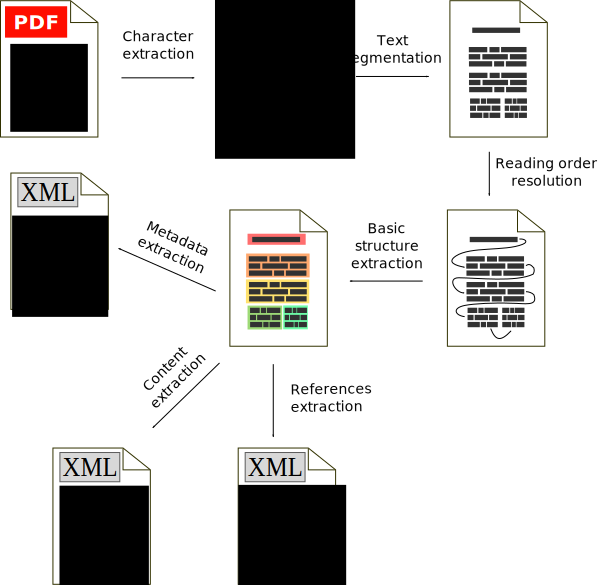
\includegraphics[width=14cm]{graphics/pipeline}
  \caption{A schematic diagram of CERMINE's workflow.}
  \label{fig:pipeline}
\end{figure}

\section{Structure extraction}
\subsection{Character extraction}\label{sec:character_extraction}
PDF document as such consists of a stream of characters, whereas position of each character in the stream doesn't have to be related, and usually is not, to its position in the text. Extraction of the characters is achieved using iText library. This part of the system was entirely implemented by Dominika Tkaczyk and will not be described in this work.
\subsection{Page segmentation}\label{sec:page_segmentation}
Page segmentation is a task of clustering a set of characters into blocks of text. Implemented system uses internally the Docstrum algorithm, described in details in \cite{O'Gorman1993}. It is a bottom-up approach based on
nearest-neighborhood clustering of connected components extracted from the document. $K$-neareast neigbours for each component are found and text lines are found based on a threshold of the angle between component centroids. Then, histograms of components spacing are used to detect inter-character distance in a word and between words. The algorithm has a set of thresholds that have to be set based on experiments with various documents. The algorithm was implemented by Krzysztof Rusek and tuned by Dominika Tkaczyk and therefore will not be described in this document in details.

\subsection{Reading order resolving}\label{sec:reading_order}
Resolution of Reading Order is a process aiming to transform text zones from a two-dimensional space (as they are laid out on the paper) to a single-dimensional space, i.e. as they are read by a human. Usually this is done by going from left to right and from top to bottom, but there are a lot of cases that made this na\"\i ve approach less efficient. This includes multi-column layout, page numbers, textual elements of figures, figures' and equations' labels.
\qquad
As already described in \cite{DominikaTkaczykPaweSzostekMateuszFedoryszakPiotrJanDendek2014}, a PDF file contains a stream of characters that undergoes processes of extraction and segmentation. This results in a list of pages consisting of zones, lines, words and chunks of text. These elements need to be put together in the same order as that would be done by a human reader.\\
To this end, a bottom-up strategy is applied: firstly characters are sorted within words and words within lines in ascending order according to X coordinate value. Afterwards, lines are sorted with Y coordinate as the key. As next we need to figure out zones' order. Below we describe a heuristic responsible for setting order of text zones Its fundamental principle was taken from \cite{ROR_source}. A schematic diagram of this phase can be found in the figure \ref{fig:reading_order}.
\begin{figure}[]
  \centering
  \includesvg[width=12cm]{graphics/ro}
  \caption{A schematic diagram of reading order resolving. Firstly, distances between text zones are calculated. Then, zones are hierarchicaly grouped according to distances between them. Finally, the tree is in-order traversed and a list of zones in created.}
  \label{fig:reading_order}
\end{figure}
\begin{enumerate}
\item For each pair of items inside a single page boundaries a free space between them is calculated. On the figure \ref{fig:reading_order} this space is ilustrated as the black area between two zones. The full implementation of the algorithm is included in the appendix \ref{appendix:ror}. Below is a detailed description of the steps taken.
	\begin{enumerate} 
	\item Formally the free space $S$ can be expressed as $S = A_d - (A_1+A_2)$, where $A_1$ and $A_2$ are areas of the two zones and $A_d$ is area of the smallest rectangle in which two objects can fit. This rectangle has to have sides parallel to the X and Y axes.
	\item To include preference for vertical clustering (and to avoid joining blocks horizontally when multi-column layouts are present) a cosine of the angle $\alpha$ between the vector $\vec{v}$ connecting two objects' geometrical centers and vector $\vec{x}$ being a projection of the vector $\vec{v}$ on the X axis is calculated. This was illustrated in the figure \ref{fig:angle_alpha}. The formula $\cos\alpha = \frac{\vec{v} \cdot \vec{x}}{|\vec{v}||\vec{x}|}$ is employed.
	\item Free space $S$ is multiplied by sum of coefficient $M$ and $\cos\alpha$. Coefficient $M$ is introduced in order to prevent situations when more than two zones have the same width and lay in-line with respect to the Y axes. Then, for each of them the calculated distance would be equal to zero. In such cases we prefer to join these two groups between which the Euclidean distance is minimized.
	\end{enumerate}
\item A list $L$ containing triples ($O_1$, $O_2$, $D$) is created (where $O_1$ and $O_2$ are zones on the page and $D$ is the distance between zones) Initially there are $\binom{N}{2}$ elements in the list.
\item List $L$ is sorted in ascending order with respect to the distance $D$. 
\item Until this list is empty, the first triple is picked (i.e. with the smallest distance $D$) and two associated objects, $O_1$ and $O_2$, are merged.
\item For each element $E$ in the $L$ recalculate the distance $D$ to the new group iff the $E$ contains $O_1$ or $O_2$ (i.e. is in form of ($O_1$, $X$, $D$) or ($O_2$, $X$, $D$)).  Insert into the list a new triple ($O_1O_2$, $X$, $D$) where $O_1O_2$ is the new group.
\item Sort the list $L$ in ascending order.
\end{enumerate}
\begin{figure}[h!]
  \centering
  \includesvg[width=8cm]{graphics/angle_alpha}
  \caption{To include preference for vertical clustering a cosine of the angle $\alpha$ between the vector $\vec{v}$ and vector $\vec{x}$ is calculated.}
  \label{fig:angle_alpha}
\end{figure}
\begin{lstlisting}[caption=Listing of the function measuring distance between two zones or zone groups.]

private double distance(BxObject obj1, BxObject obj2) {

    double x0 = Math.min(obj1.getX(), obj2.getX());
    double y0 = Math.min(obj1.getY(), obj2.getY());
    double x1 = Math.max(obj1.getX() + obj1.getWidth(),
            obj2.getX() + obj2.getWidth());
    double y1 = Math.max(obj1.getY() + obj1.getHeight(),
            obj2.getY() + obj2.getHeight());
    double dist = ((x1 - x0) * (y1 - y0) - obj1.getArea() - obj2.getArea());

    double obj1CenterX = obj1.getX();
    double obj1CenterY = obj1.getY() + obj1.getHeight() / 2;
    double obj2CenterX = obj2.getX();
    double obj2CenterY = obj2.getY() + obj2.getHeight() / 2;

    double obj1obj2VectorCosineAbs = Math.abs((obj2CenterX - obj1CenterX) / Math.sqrt((obj2CenterX - obj1CenterX) * (obj2CenterX - obj1CenterX) + (obj2CenterY - obj1CenterY) * (obj2CenterY - obj1CenterY)));
    final double M_COEFF = 0.5;
    return dist * (M_COEFF + obj1obj2VectorCosineAbs);
}
\end{lstlisting}
\section{Initial zone classification}
After the stages described in sections \ref{sec:character_extraction}, \ref{sec:page_segmentation} and \ref{sec:reading_order} the document can undergo the two phases of classification. Firstly, all the zones are classified to one of the four general classes: \verb+METADATA+, \verb+REFERENCES+, \verb+BODY+ and \verb+OTHER+. After this stage, more specific classifiers and algorithms can perform finer-grained analysis on the zones falling into each class. Semantics of these classes is as following
\begin{itemize}
\item \verb+METADATA+ contains all the data which do not constitute the proper content. This includes publication elements such as: title, author name, affiliation, bibliographic informations, abstract etc.
\item \verb+BODY+ contains text of the publication. This includes the chapters, figures, tables, equations, plots, acknowledgments, headings, contribution statements, conflict statements and attachments.
\item \verb+REFERENCES+ contains article's references,
\item \verb+OTHER+ contains misclassified zones and page numbers. It is a result of a non-ideal dataset, being tagged only to some extent. When training the classifier, those unclassified zones are labeled as \verb+OTHER+. This in turn introduces some kind on additional noise. We decided that it is better to exclude a handful of zones from the further processing (i.e. classify them as \verb+OTHER), than to classify them incorrectly to one of the remaining classes. Employed dataset contains 3.6\% of unknown labels, therefore we might expect a similar number of zones classified to \verb+OTHER+ in the classifier's output.
\end{itemize}
\quad
Initial classification is node using an SVM classifier with the parameters given in the table \ref{tab:classifier_parameters}.
\begin{table*}
\centering
\begin{tabular}{@{}rrr@{}}
\toprule
& initial & metadata \\
\midrule
SVM type & C\_SVC & C\_SVC \\ 
kernel type & polynomial & polynomial \\
$\gamma$ & $\frac{1}{8}$ & $\frac{1}{8}$ \\ 
$C$ & 8 & 8 \\
$coef_0$ & 0.5 & 0.5 \\
$degree$ & 3 & 3 \\
\bottomrule
\end{tabular}
\label{tab:classifier_parameters}
\caption{Parameters used in the final training of both classification stages}
\end{table*} 
\section{Metadata classification}
Once the initial coarse-grained classification is done, we employ a second classifier which is specialized in classifying metadata, i.e. those zones, which initially got the \verb+METADATA+ label. This class contains 19 sub-labels:
\begin{itemize}
    \item \textbf{abstract} - document's abstract, usually one or more zones placed in the first page of the document;
    \item \textbf{acknowledgments} - sections containing information about document's acknowledgments or funding;
    \item \textbf{affiliation} - authors' affiliations sections, which sometimes contain contact information (emails, addresses) as well;
    \item \textbf{author} - a list of document's authors,
    \item \textbf{bib\_info} - zones containing all kinds of bibliographic information, such as journal/publisher name, volume, issue, DOI, etc.; often includes pages' headers or footers; headers and footers containing document's title or author names are also labelled as bib\_info;
    \item \textbf{body\_content} - the text content of the document, contains paragraphs and section titles;
    \item \textbf{conflict\_statement} - conflict statement declarations;
    \item \textbf{copyright} - copyright or license-related sections;
    \item \textbf{correspondence} - the authors' contact information, such as emails or addresses;
    \item \textbf{dates} -important dates related to the document, such as received, revised, accepted or published dates;
    \item \textbf{editor} - the names of the document's editors;
    \item \textbf{equation} - equations placed in the document;
    \item \textbf{figure} - zones containing figures' captions and other text fragments belonging to figures;
    \item \textbf{glossary} - important terms and abbreviations used in the document;
    \item \textbf{keywords} - keywords listed in the document;
    \item \textbf{page} number -zones containing the numbers of pages;
    \item \textbf{table} - the text content of tables and table captions;
    \item \textbf{title} - the document's title;
    \item \textbf{title\_author} - zones containing both document's title and the list of authors;
    \item \textbf{type} -the type of the document, usually mentioned on the first page near the title, such as ``research paper'', ``case study'' or ``editorial'';
    \item \textbf{unknown} - used for all the zones that do not fall in any of the above categories.
\end{itemize}
\section{Optimization of classifiers' parameters} 
As already described in section \ref{sec:svm} CERMINE uses internally the SVM algorithm to classify  
\section{References extraction}
\section{Text extraction}
\section{Feature selection}
In both stages of classification we employed a set of features including almost one hundred elements. In appendix \ref{appendix:features} there is a detailed description of how their values are calculated. Briefly, they can be divided into following groups:
\subsubsection{Sequence features}
This group contains only two features: \textit{PreviousZoneFeature} and \textit{LastButOneZoneFeature}. It leverages the fact that the zones are classified after the process of reading order resolution is done. The features contain numerical value of two previous labels. In turn, this allows to incorporate sequence information into classification, which is not done in SVM by design (as opposed to for instance Hidden Markov Model).
\subsubsection{Formatting features}
This group of features contains information about graphical properties of text. It can be very helpful while certain elements in scholarly publications are usually typed with bigger font size
\subsubsection{Layout features}
These features encode information about graphical layout on the page. This includes properties of the zone itself (e.g. \textit{WidthFeature}, \textit{HeightFeature}, \textit{LineMeanWidthFeature}) as well as features of the area between text zones (e.g. \textit{HorizontalRelativeProminenceFeature},\textit{VerticalRelativeProminenceFeature}, \textit{IsHighestOnThePage}, \textit{IsGreatestOnThePage}, \textit{DistanceFromNearestNeighbourFeature}). 
\subsubsection{Semantic features}
This group of features encodes appearence of certain key-words that very often characterize certain parts of articles written with scientific english, e.g. ``keywords'', ``terms'', ``distributed'', ``reproduction'', ``open'', ``commons'', ``license'', ``creative'', ``copyright'', ``cited'', ``distribution'', ``access'', ``references'', ``author'', ``bibliography'', ``figure'', ``table'', ``editor'', ``email'', ``correspondence'', ``address'', ``abstract'', ``author details'', ``university'', ``department'', ``school'', ``institute'', ``affiliation'', ``affiliation'', ``research article'', ``review article'', ``editorial'', ``review'', ``debate'', ``case report'', ``research'', ``original research'', ``methodology'', ``clinical study'', ``commentary'', ``article'', 
 ``hypothesis'', .
\subsubsection{Special features}
This group contains features that do not fit other groups described above. This includes e.g. \textit{IsAnywhereElseFeature}, \text{BracketCountFeature}, \text{CharCountFeature}, \text{CommaCountFeature}.

\section{Learning process}
\subsection{Model cross-validation}
\chapter{Classification}
Below we present the whole workflow leading from training data to a working tool capable of classifing unknown data.
\section{Classification training workflow}
\subsection{Generating samples}
TrueViz documents are an input for the classification training workflow. As depicted in \ref{DUPA} they consists of text together with its geometrical properties and class. The zones are used to generate training samples, which are values of plethora of features for particular zones together with the classification information. Semantics of the feature values is as following: \textit{if the final classifier gets an input that has the same values of features, it should be classified in the same way as the training sample}. The role of a classifier is to extrapolate in a compact way data from the training samples to unseen cases.
\subsection{Data scaling}
A very important step towards learning a classifier is scaling of the input data. The main motivation behin that, as mentioned in \cite{Chih-WeiHsu2010}, is not to allow variables in greater numerical ranges to dominate those in smaller numerical ranges. What is more, large values might cause numerical problems. One has to take into account that the closer to zero floating point variables are, the more precisely are they represented. Scaling recommended by \cite{Chih-WeiHsu2010} is in range [-1, +1] or  [0, 1]. The latter is used in CERMINE. Obviously, both learning and testing data have to be scaled using the same transformation. Thus, it is necesary to retain extreme values encountered in learning process.
In CERMINE scaling for learning purposes was realized with \verb+svm-scale+, a software tool delivered together with the \verb+libsvm+ package.
\subsection{Data sampling}
When the decision classes are unequally represented in the training data. The approaches used to deal this problem can be divided into three groups (\cite{Choi}):
\begin{enumerate}
\item Changing class distribution by modyfing the data itself in order to rebalance it. It can be reached by either getting rid of samples from over-represented classes or by cloning samples from the under-represented classes. The former can greatly reduce the time spent on the optimization phase. The latter prohibits not common samples from falling out of the training set, making the resulting classifier more versatile.
\item Adjusting the classifier itself by applying different misclassification costs for different classes. These costs might be for instance inversely linear to number of samples in each class.
\item Ensamble learning methods, i.e. using multiple classifiers learnt with multiple training data and then combining output of the classifier, for instance by a simple voting.
\end{enumerate}
In CERMINE two first of the mentioned approaches were tested and the second one is included in the final code.
\subsection{Transformation to svmlight format}
Various SVM packages, including libsvm, require that the data are represented as vectors of real numbers. Thus, if the data contains cathegorical attributes (such as \verb+red+, \verb+green+, \verb+blue+ or \verb+big+, \verb+small+) they have to be converted to numerical values. There are two common approached to this problem:
\begin{itemize}
\item Using a single value to encode the category. This can be very easily implemented by using the integer value behind enumeration in C implementation
\item Using N different numbers to represent a category with N possible values. According to \cite{Chih-WeiHsu2010}, this approach yields more stable results
\end{itemize}
\qquad
Svmlight format is a text file format that requires every training sample to be in a separate line (thus, they must be split with new line characters). Each line consists of a certain number of fields separated with white signs, e.g. spaces. Each line has to begin with a number representing the decision class followed by feature values. There are no constrains regarding encoding of the decision classes, as long as this encoding is coherent. Feature values have a form of $f_n:v_n$, where $f_n$ is the feature number and $v_n$ is its value. Not every feature has to be listed, but only these whose values are non-zero. This format is beneficial for the scenarious where features are sparse.

\subsection{Parameter optimization}
\label{sec:svm_optimization}
It impossible to tell \textit{a priori} which kernel function is the most appropriate for the given training data. There are kernels that behave usually well (and RBF is one of them) and these should be a choice when the learning process is constained by time.

SVM classifier have a handful of free variables and kernel type is one of them. In general, when optimizing a classifier one has to find a triple $(K, C, \gamma)$ that maximizes classifier's accuracy for the given training data. In this triple $K$ is the kernel type, $C$ is a generic cost of misclasifying data and $\gamma$ is a kernel parameter. One of the techniques of obtaining them is an extensive parameter space search by checking classifier's accuracy in every point on a parameter grid. Commonly this kind of search is called \textit{grid search} and does not allow to omit any of the points in the parameter space without a risk of missing a possibly optimal point.

For every point in the space a $k$-fold crossvalidation is applied. It means that for a set of parameters the training set is divided into $k$ subsets, each of equal or nearly-equal size. At every step $k-1$ of these subsets constitue the training set and the remaining $k$-th set is treated as the uknown data employed to verify correctness of the trained classifier. The trained classifier is applied to classification of the pseudo-unknown data and finally their \textit{de facto} is compared to the output of the classification. After $k$ iterations the mean efficiency is calculated and it serves as a criterium for evauluating the current $(K, C, \gamma)$ triple.


In the case of CERMINE grid search was performed on 16'384 samples from GROTOAP2. The training set was limited to this size to limit to make possible evaluation with reasonable time constraints. For both classifiers four kernels were tested with $log_{10}C$ and $log_{10}\gamma$ varying with a unit step in range $[-5,15]$ and $[-15,3]$ respectively, resulting in 399 points tested for every classifier. In total there were 3192 ($=399\cdot4\cdot2$) points tested in the first pass, which yielded candidates for accuracy maxima. Later, a fine-grained search was lead with the best kernels (both RBF) around the candidates for maximum in distance of $1dB$ with a step equal to 0.25, resulting in additional 81 points being checked for each of the classifier. Results of this procedure are presented in the figures \ref{fig:initial_linear}, \ref{fig:initial_poly}, \ref{fig:initial_rbf}, \ref{fig:initial_sigmoid}, \ref{fig:initial_fine}, \ref{fig:meta_linear}, \ref{fig:meta_poly}, \ref{fig:meta_rbf}, \ref{fig:meta_sigmoid} and \ref{fig:meta_fine}. Optimal obtained parameters for the classifiers are presented in the table \ref{tab:classifier_parameters}.

\begin{table*}[h!]
\centering
\begin{tabular}{@{}rrr@{}}
\toprule
& Initial classifier & Metadata classifier \\
\midrule
SVM type & C\_SVC & C\_SVC \\ 
kernel type & RBF & RBF \\
$\gamma$ & -4.0 & -2.5 \\ 
$C$ & 2.75 & 4.25 \\
$coef_0$ & 0.5 & 0.5 \\
\midrule
mean accuracy & 93.66 & 86.98 \\
\bottomrule
\end{tabular}
\caption{Results of the grid search in parameter space for the initial and metadata classifiers.}
\label{tab:classifier_parameters}
\end{table*}

\begin{center}
\begin{figure}
	\centering
  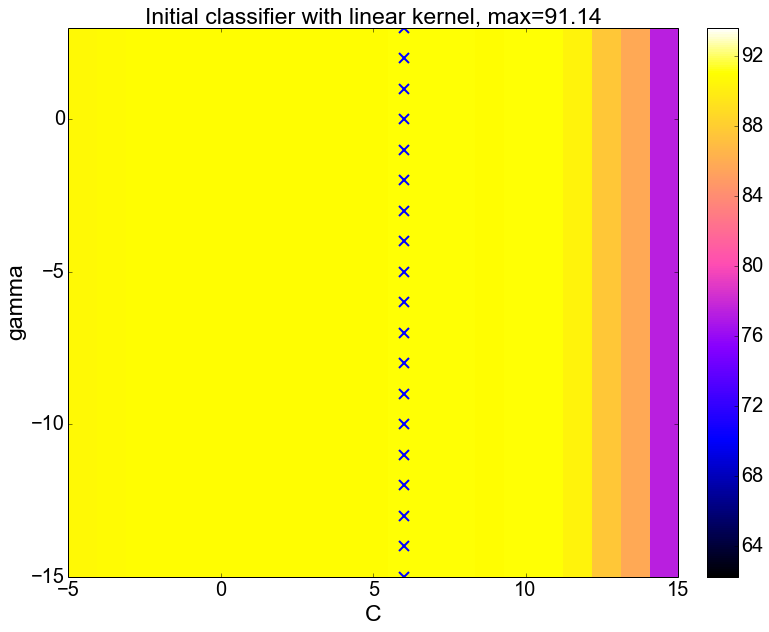
\includegraphics[width=1\textwidth]{plots/init_linear}
  \caption{Grid search over two-dimensional parameter space ($C$, $\gamma$) with linear kernel for the initial classifier. The maximal accuracy in 5-fold cross-validation is equal to 91.14 and is found for $log_{10}C=6$}
  \label{fig:initial_linear}
\end{figure}
\begin{figure}
\centering
  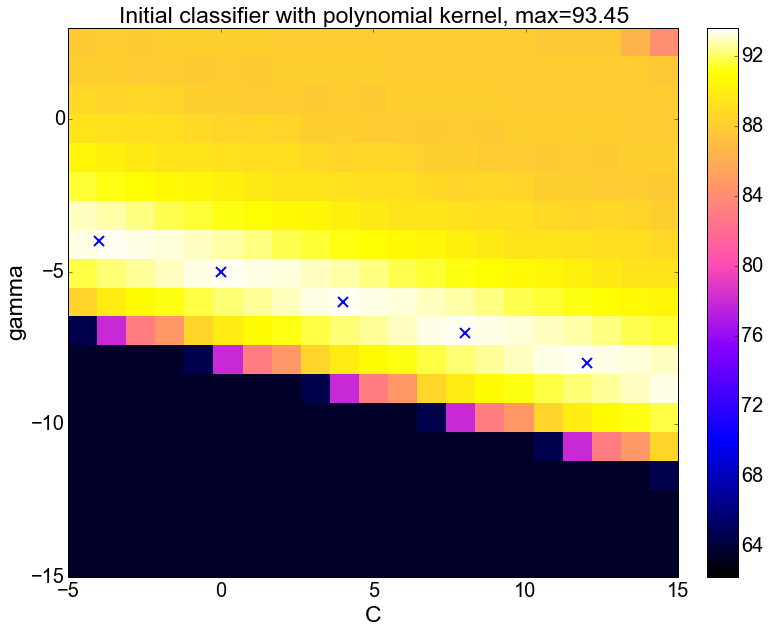
\includegraphics[width=1\textwidth]{plots/init_poly}
  \caption{Grid search over two-dimensional parameter space ($C$, $\gamma$) with polynomial $4^{th}$-degree kernel for the initial classifier. In the investigated interval there are 5 maxima. Classifier accuracy over 5-fold validation is equal to 93.45 and is found for instance for $log_{10}C=3$ and $log_{10}\gamma=-7$.}
  \label{fig:initial_poly}
\end{figure}

\begin{figure}
	\centering
  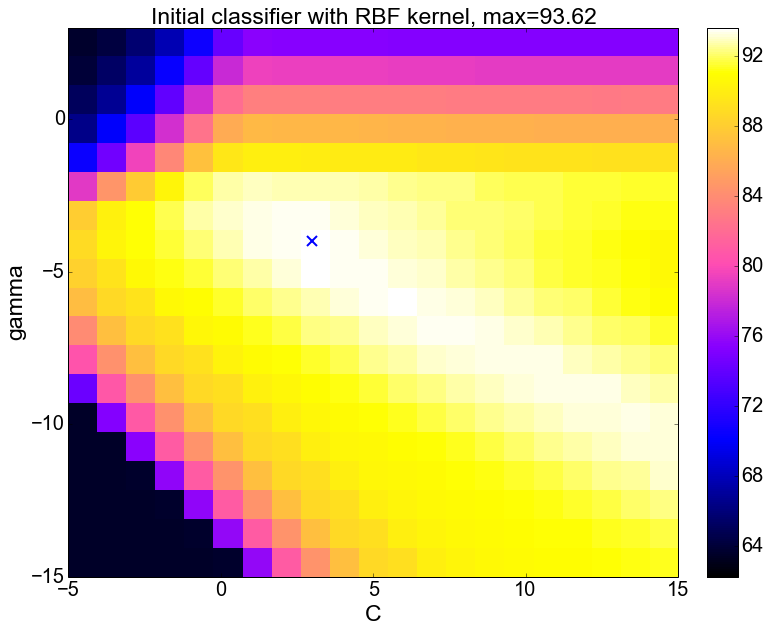
\includegraphics[width=1\textwidth]{plots/init_rbf}
   \caption{Grid search over two-dimensional parameter space ($C$, $\gamma$) with a radial-basis function kernel for the initial classifier. The maximal accuracy in 5-fold cross-validation is equal to 93.62 and is found for $log_{10}C=3$ and $log_{10}\gamma=-4$. This was the highest accuracy found in the first pass. The second pass refined the maximum around the initial result.}
   \label{fig:initial_rbf}
\end{figure}
\begin{figure}
	\centering
  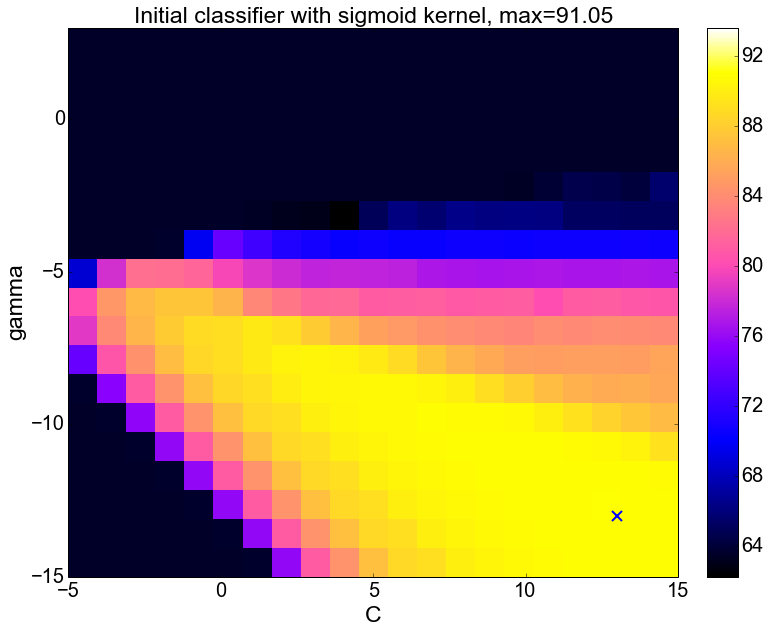
\includegraphics[width=1\textwidth]{plots/init_sigmoid}
  \caption{Grid search over two-dimensional parameter space ($C$, $\gamma$) with a sigmoid kernel for the initial classifier. The maximal accuracy in 5-fold cross-validation is equal to 91.05 and is found for $log_{10}C=13$ and $log_{10}\gamma=-13$}

  \label{fig:initial_sigmoid}
\end{figure}
\begin{figure}
	\centering
  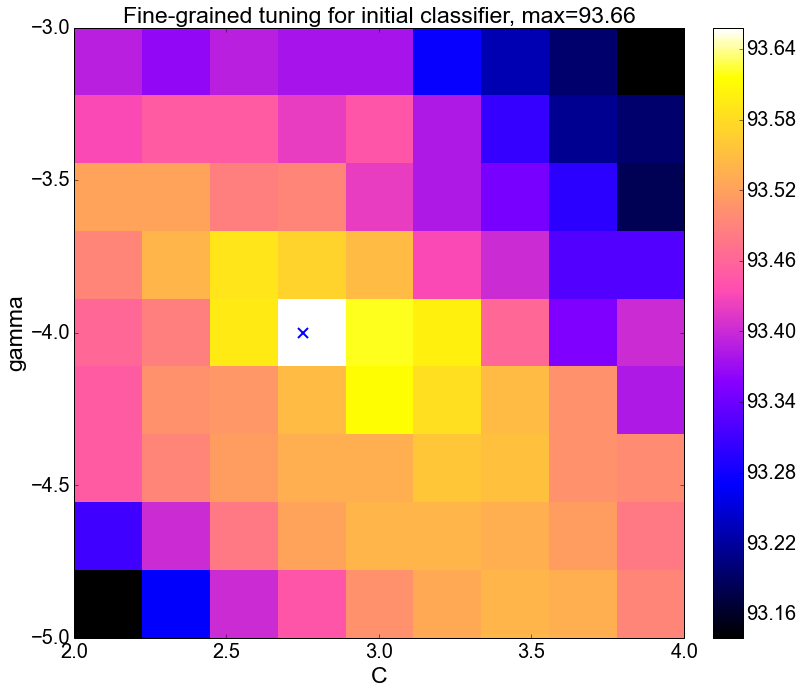
\includegraphics[width=\textwidth]{plots/init_fine}
  \caption{Fine-grain search around initial classifier with RBF kernel for the initial classifier (the color-mapping scheme is not coherent with the previous plots). Initial coarse-grain search yielded the maximum in ($log_{10}C=3$, $log_{10}\gamma=-4$) equal to 93.62. This search refines the search with $log_{10}step=0.25$ yielding maximum in ($log_{10}C=2.75$, $log_{10}\gamma=-4$) equal to 93.66. This parameters are used for training of the final classifier.}
  \label{fig:initial_fine}
\end{figure}
\begin{figure}
	\centering
  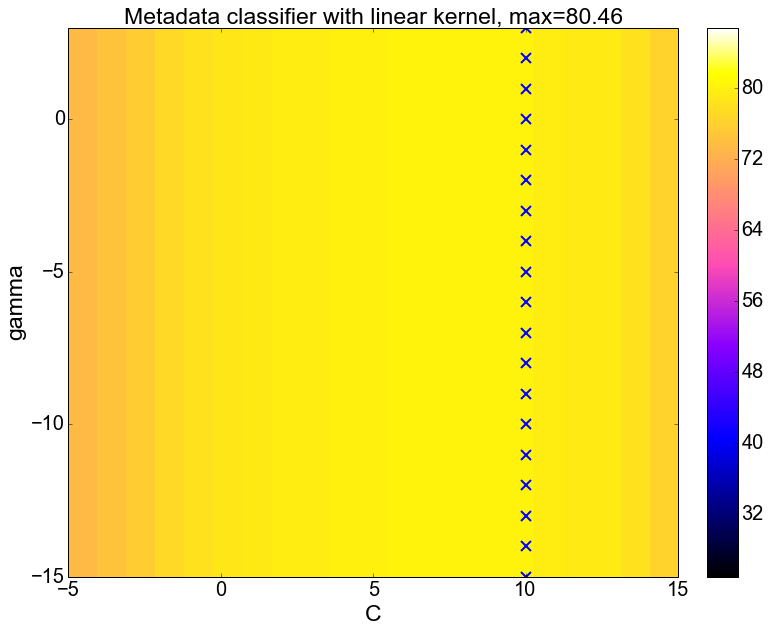
\includegraphics[width=\textwidth]{plots/meta_linear}
  \caption{Grid search over two-dimensional parameter space ($C$, $\gamma$) with linear kernel for the metadata classifier. The maximal accuracy in 5-fold cross-validation is equal to 80.46 and is found for $log_{10}C=19$}
  \label{fig:meta_linear}
\end{figure}
\begin{figure}
\centering
  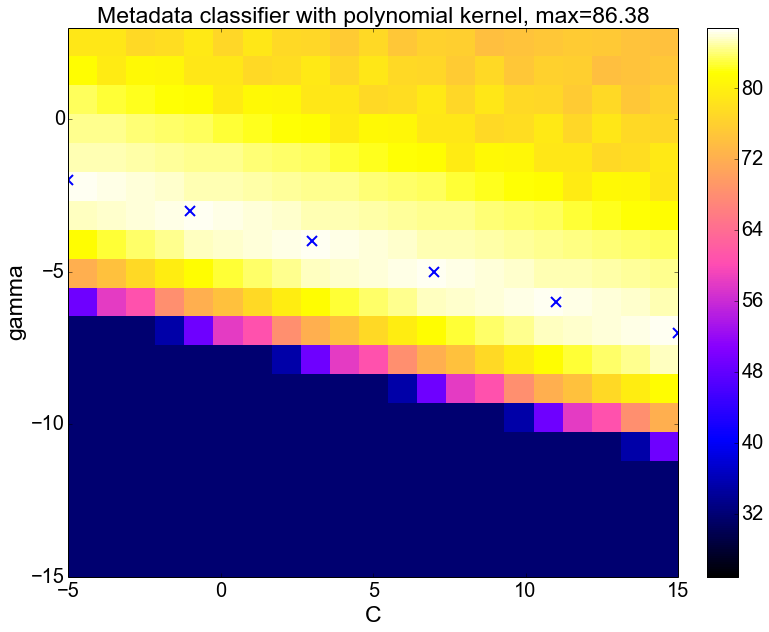
\includegraphics[width=\textwidth]{plots/meta_poly}
  \caption{Grid search over two-dimensional parameter space ($C$,$\gamma$) with polynomial $4^{th}$-degree kernel for the metadata classifier. In the investigated interval there are 5 maxima. Classifier accuracy over 5-fold validation is equal to 86.38 and is found for instance for $log_{10}C=7$ and $log_{10}\gamma=-5$.}
  \label{fig:meta_poly}
\end{figure}

\begin{figure}
	\centering
  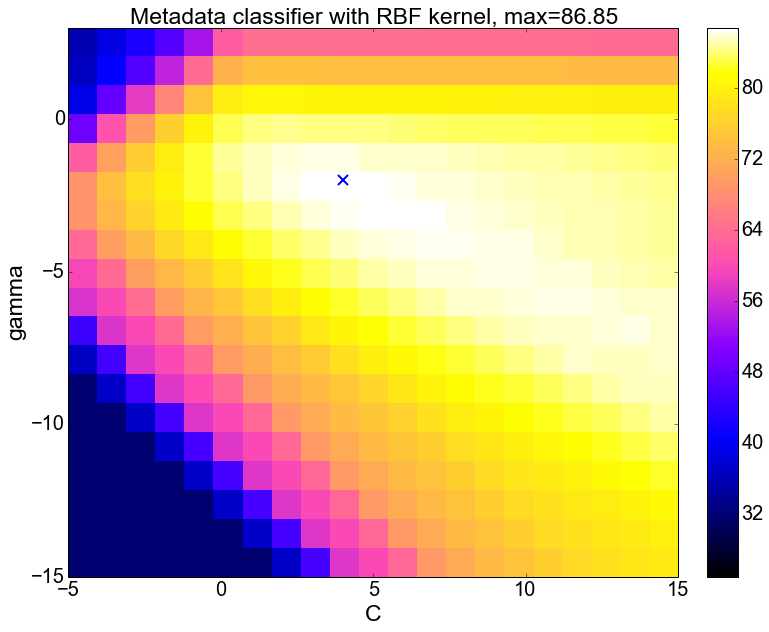
\includegraphics[width=\textwidth]{plots/meta_rbf}
   \caption{Grid search over two-dimensional parameter space ($C$, $\gamma$) with a radial-basis function kernel for the metadata classifier. The maximal accuracy in 5-fold cross-validation is equal to 86.85 and is found for $log_{10}C=4$ and $log_{10}\gamma=-2$. This was the highest accuracy found in the first pass. The second pass refined the maximum around the initial result.}
  \label{fig:meta_rbf}
\end{figure}
\begin{figure}
	\centering
  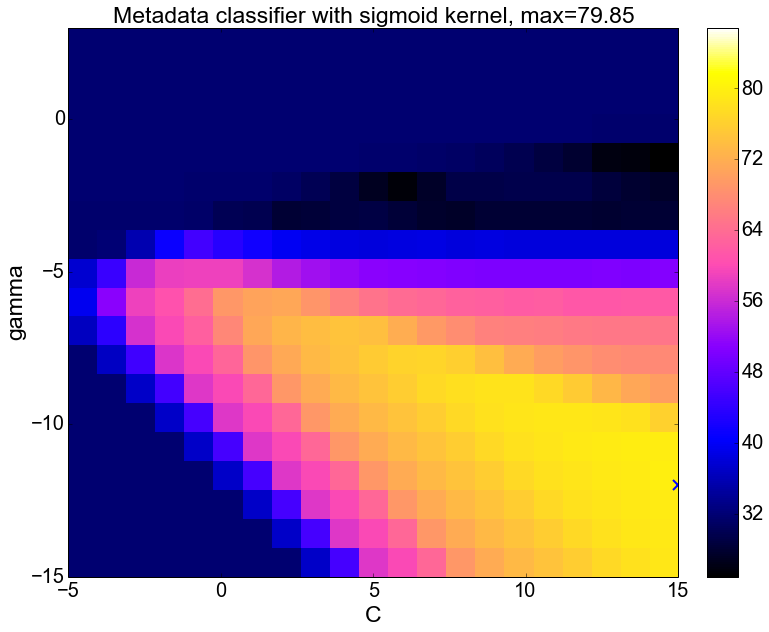
\includegraphics[width=\textwidth]{plots/meta_sigmoid}
  \caption{Grid search over two-dimensional parameter space ($C$, $\gamma$) with a sigmoid kernel for the initial classifier. The maximal accuracy in 5-fold cross-validation is equal to 79.85 and is found for $log_{10}C=15$ and $log_{10}\gamma=-12$}
  \label{fig:meta_sigmoid}
\end{figure}
\begin{figure}
	\centering
  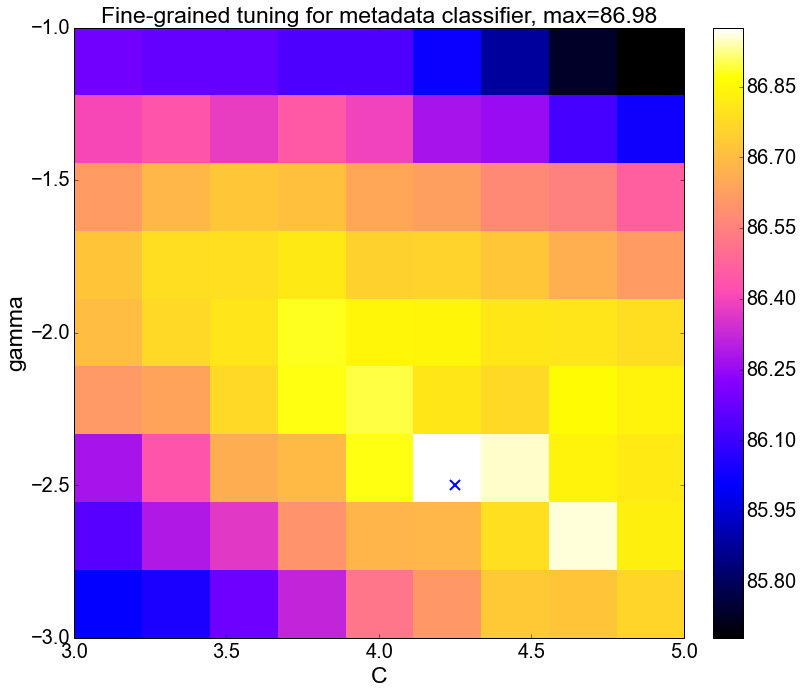
\includegraphics[width=\textwidth]{plots/meta_fine}
  \caption{Fine-grain search around initial classifier with RBF kernel for the metadata classifier (the color-mapping scheme is not coherent with the previous plots). Initial coarse-grain search yielded the maximum in ($log_{10}C=4$, $log_{10}\gamma=-2$) equal to 86.85. This search refines the search with $log_{10}step=0.25$ yielding maximum in ($log_{10}C=4.25$, $log_{10}\gamma=-2.5$) equal to 86.98. This parameters are used for training of the final classifier.}
  \label{fig:meta_fine}
\end{figure}
\end{center}

\subsection{Training of the final classifier}
After the optimal parameters have been found using a grid search, we train the classifiers to perform the final evaluation. This process is characterized in the appendix \ref{appendix:training_workflow}. To this end, we used classes \verb+SVMInitialZoneClassificationEvaluator+ and \verb+SVMMetadataClassificationEvaluator+ that build the classifier and perform cross-validation at a time. Its results are presented in the chapter \ref{chapter:evaluation}.

\section{Feature selection}
In both stages of classification we employed a set of features including almost one hundred elements. In appendix \ref{appendix:features} there is a detailed description of how their values are calculated. Briefly, they can be divided into following groups:
\subsubsection{Sequence features}
This group contains only two features: \textit{PreviousZoneFeature} and \textit{LastButOneZoneFeature}. It leverages the fact that the zones are classified after the process of reading order resolution is done. The features contain numerical value of two previous labels. In turn, this allows to incorporate sequence information into classification, which is not done in SVM by design (as opposed to for instance Hidden Markov Model).
\subsubsection{Formatting features}
This group of features contains information about graphical properties of text. It can be very helpful while certain elements in scholarly publications are usually typed with bigger font size
\subsubsection{Layout features}
These features encode information about graphical layout on the page. This includes properties of the zone itself (e.g. \textit{WidthFeature}, \textit{HeightFeature}, \textit{LineMeanWidthFeature}) as well as features of the area between text zones (e.g. \textit{HorizontalRelativeProminenceFeature},\textit{VerticalRelativeProminenceFeature}, \textit{IsHighestOnThePage}, \textit{IsGreatestOnThePage}, \textit{DistanceFromNearestNeighbourFeature}). 
\subsubsection{Semantic features}
This group of features encodes appearence of certain key-words that very often characterize certain parts of articles written with scientific english, e.g. \textit{keywords}, \textit{terms}, \textit{distributed}, \textit{reproduction}, \textit{open}, \textit{commons}, \textit{license}, \textit{creative}, \textit{copyright}, \textit{cited}, \textit{distribution}, \textit{access}, \textit{references}, \textit{author}, \textit{bibliography}, \textit{figure}, \textit{table}, \textit{editor}, \textit{email}, \textit{correspondence}, \textit{address}, \textit{abstract}, \textit{author details}, \textit{university}, \textit{department}, \textit{school}, \textit{institute}, \textit{affiliation}, \textit{affiliation}, \textit{research article}, \textit{review article}, \textit{editorial}, \textit{review}, \textit{debate}, \textit{case report}, \textit{research}, \textit{original research}, \textit{methodology}, \textit{clinical study}, \textit{commentary}, \textit{article}, 
 \textit{hypothesis}, .
\subsubsection{Special features}
This group contains features that do not fit other groups described above. This includes e.g. \textit{IsAnywhereElseFeature}, \text{BracketCountFeature}, \text{CharCountFeature}, \text{CommaCountFeature}.
\chapter{Dataset}
\section{Motivation}
Despite a strong need of performing automated analyses of scholarly publications, there are no big and reliable datasets of annotated publications available publicly. Such a dataset would greatly facilitate the process of building a classifier to perform the processes of metadata extraction, which, even when boiled down to scientific publishing, is error prone and not trivial. By far this is caused by two factors:
\begin{itemize}
\item scientific publishing is inherently \textit{blessed} by richness of layouts, formats and designs. No one is to be blamed for this variety which is to the most extreme degree natural. Any tool that aims to be reliable needs to take this diversity of styles into account.
\item PDF, being a \textit{de facto} standard in the scientific publishing, is a format designed to carry content as it displayed. However, it is not suitable for carrying metadata. Its main design goal was to hold geometrical metadata allowing a faithful reproduction of the source document's display with different tools and platforms. It holds no relevant metadata and the structure of the input document is broken down to the level of single characters
\end{itemize}
Each publisher or even each journal follows its own layout. For instance, in the Open Access subset of PubMed Central there are more than 800 publishers, each of them very likely following a different layout. We need to keep in mind that the articles included there are biology-related which is only a fraction of scientific publishing. It's safe to assume that there are thousands of publishers worldwide. We decided to put together a diverse set of articles that could serve as a basis for automatic approach for content analysis. 

\section{Related work}
The vast majority of the data sets publicly available is based on images, i.e. there are no born-digital documents available. As an example here we might give MARG, which contains scanned first pages of biomedical articles. This makes its usability in our case very limited. PRImA is a data set containing images of various documents, whose category goes beyond scientific publishing. Again, these are images which aren't helpful in case of chosen architecture. Conversely, The UW-III data set contains both articles' images and born-digital data. It is not available freely, though. What is more, we preferred to focus in our work on pure scientific articles as those are the target input of the designed system.
\section{Pubmed database}
Pubmed \cite{Pubmed} is a collection of more than 24 millions articles from MEDLINE, life science journals and online books maintained by the US National Library of Medicine. This collection is digitized which means that the articles are stored in form of PDF files and can serve as a source of full texts without a need for performing Optical Character Recognition. 
The PMC Open Access Subset (abbreviated to PMC-OAS) is a part of the collection of Pubmed central available publicly with any fees. These articles are kept protected by copyrights, but can be used under the Creative Commons license that allows for more liberal usage of the resources. For the time of creating this report (June 2014) there were more than 400,000 articles available.
\section{Dataset creation}
With very limited budget it is clearly impossible to create a rich set of annotated articles by human means. A predecessor of the thereafter described data set was created at ICM in \cite{Tkaczyk2012}. GROTOAP (\textit{GROund Truth for Open Access Publications}) created there is a collection of 113 articles in digital form with corresponding ground-truth files. This data set was created semi-automatically. First, a handful of articles was tagged manually and supplied to a predecessor of CERMINE as a training input. Then, the remaining part of articles was tagged by the trained classifier and corrected by experts later on, guaranteeing high precision and accuracy.

Its downside was that the included articles cover not more than 15 different layouts, which is certainly not enough when aiming to build a tool applicable to the whole spectrum of publishers and layouts. Initial tests have proven that this data set did not provide sufficient diversity for the classifier to perform well enough. This is why it was decided to create a dataset, called GROTOAP2, that could serve as a base for classifiers.

\section{GROTOAP2 properties}
GROTOAP2 is made of ground-truth files in TrueViz format, which extends XML, containing publications' content structured hierarchically and tagged according to its role. This is accompanied by geometrical data on 4 levels of granularity: text zone, text line, word and character whose role is to reflect how the content should be displayed according to the PDF files. Since function of a piece of text can be distinguished not only by the text itself, but also by its appearance, i.e. the geometrical features, a dataset applicable for training a classifier must preserve the information related to dimensions and positions of the objects.

In GROTOAP2 there are in total 13210 articles made of 119334 pages and 1640973 zones coming from 208 different publishers and 1170 different journals. The data set is distributed under the CC-BY license and can be downloaded from the server of Center for Open Science \cite{CeON}. It is available together with a list of URLs for the corresponding PDF files (which are not included in the data set itself) and scripts downloading both input XMLs and the PDFs.

\section{The methodology of creating GROTOAP2}
As stated before, it was assumed that GROTOAP2 has to be based on open access articles. Pubmed was chosen as source of input data, as a great majority of contained articles is associated with extracted metadata. Sometimes their quality might be put in doubt, but the process was designed to automatically filter them out. The method presented here is scalable to immense sets as the human factor was ruled out.

Each article in the Pubmed dataset comes as a tarball containing the article itself (in PDF file format), a metadata file (in XML file format) and possible some resource files, mainly including pictures extracted from the PDF. A sample content of a metadata XML is showed in the listing \ref{lst:pmc_xml}. A complete description of possible elements can be found in \cite{PubmedXML}.
\lstinputlisting[label={lst:pmc_xml},caption={Sample content of a PUBMED XML file},basicstyle=\scriptsize,language=XML]{samples/pubmed_sample.xml}



The general strategy for creating ground-truth files out of the PMC-OAS was to match content of the metadata files to blocks of text extracted and segmented from the provided PDF files resulting in a tagged TrueViz file. This allowed us to mix together both data, metadata and geometric properties of the articles. \

textbf{The role played by a given document fragment can be deduced not only from its text content, but also from the way the text is displayed for the readers. As a result, document zone classifier can benefit a lot from using not only the text content of objects, but also geometric features, such as object dimensions, positions on the page and in the document, formatting, object neighborhood, distance between objects, etc. A dataset useful for training such a classifier must therefore preserve the information related to object size, position and distance.}

PMC-AOS metadata files are not perfect, though. Full understanding of their structure was achieved by thorough and laborious manual analysis of many randomly picked sample files. There are many situations that one has to take into account:
\begin{itemize}
\item structure of the documents varies between documents,
\item random fields might be missing or be incomplete,
\item same content (e.g. article's title) might be located under different paths, e.g. contributor's e-mail address might be found under \verb+/article/front/article-meta/contrib-group/contrib/email+ or \verb+/article/front/article-meta/contrib-group/contrib/address/email+.
\item same content might have different level of granularity, e.g. editor's name might be given as a flat string, whereas author's name might be divided into surname and given names,
\item elements of the same kind be found under different parents, e.g. figures might be located in \verb+/article/floats-wrap//fig+, \verb+/article/floats-group//fig+, \verb+/article/back//fig+, \verb+/article/body//fig+, \verb+/article/back/app-group//fig+
\end{itemize}
As being said, we created the data set in an automatic way (\cite{DominikaTkaczykPaweSzostek2014}):
\begin{enumerate}
    \item First, a large set of files was downloaded from Open Access Subset of PubMed Central. We obtained both source articles in PDF and corresponding NLM files containing metadata, full text and references.
    \item PDF files were automatically processed by tools provided by CERMINE and their hierarchical geometric structure along with the natural reading order was constructed.
    \item The text content of every extracted zone was compared to labeled data from corresponding NLM files, which resulted in attaching the most probable labels to zones.
    \item Files containing a lot of zones with unknown labels, that is zones for which the automatic labeling process was unable to determine the label, were filtered out.
    \item A small random sample of the remaining documents was inspected by a human expert. We were able to identify a number of repeated problems and errors and develop heuristic-based rules to correct them.
    \item From the corrected files the final dataset was chosen randomly.
\end{enumerate}

We use xpath to extract text entries from predefined paths. These paths are common for the documents in the Pubmed dataset. Each path is mapped to a label in our labeling system. The task consists in finding a mapping between NLM entries and PDF zones, so that each zone could obtain a label dependent on its path in the NLM file.

For each pair \verb+(pdf_zone, nlm_entry)+ Smith-Waterman distance
is calculated. Afterwards, for each zone a set of different approaches are followed in order to assign a correct label:
\begin{enumerate}
\item Take NLM entry with the highest ratio of SW distance to the number of tokens. If both PDF zone and NLM entry are not empty and their size expressed in number of tokens is comparable (ratio not smaller than 0.7) and length of the common substring constitutes more than 70\% of the NLM entry, then assign corresponding label,
\item if the previous approach failed, take the entry with the highest SW distance. If the length of the common substring is bigger than 50\% of the number of tokens in the PDF zone, then assign corresponding label,
\item if the previous approaches failed, a \textit{cumulative} distance is calculated. This makes it possible to assign a label to these zones that form together one NLM entry, but were segmented into several parts. This applies mostly to \verb+BODY+ zones. For each and each entry and each zone is calculated. For each zone these values are aggregated by summing them up. From all the cumulative distance the biggest one is taken. If it is greater than 0.5, the corresponding label is assigned.
\end{enumerate}
\section{Filtering}
After the matching stage we obtained initial set of TrueViz files whose quality was very diverse, i.e. spanning from fully labeled to almost unlabeled. There are two reasons for that:
\begin{figure}[ht!]
  \centering
  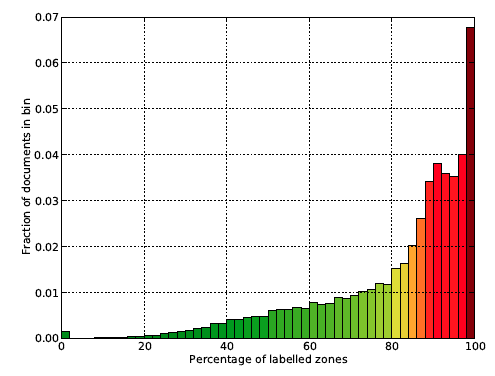
\includegraphics[width=12cm]{plots/zone_coverage_grotoap2}
  \label{fig:trueviz_match_histogram}
\end{figure}
\begin{enumerate}
\item NLM files in PMC vary in quality. Those with less detailed metadata resulted in barely labeled TrueViz files,
\item with certain layouts our segmentation algorithm was failing, producing very finely-grained text zones with just a handful of letters each. In these cases it was barely possible to match NLM metadata with the actual text, what again lead to sparsely labeled TrueViz files. 
\end{enumerate}
In order to assure good quality of the final set we needed to filter out documents with TrueViz files of bad quality. In the figure \ref{fig:trueviz_match_histogram} one can see a distribution of documents with a given fraction of labeled zones.
Based on this distribution we decided to keep these documents having the percentage of labeled zone equal or greater than 90\%.

\section{TrueViz file format}
We decided to choose TrueViz file format as the data set's main data format. This was to maintain the choice taken when working on GROTOAP data set. The motivation behind this choice is discussed in details in \cite{Tkaczyk2012}. TrueViz is a plain text file based on the XML format that holds in an extremely inefficient way the content of a document together with its geometrical properties and classification metadata. An example of a dumb file containing a single character is shown on the listing \ref{lst:trueviz_sample}.
\lstinputlisting[label={lst:trueviz_sample},caption={Sample content of a TrueViz file with one letter of content - \textit{F}},basicstyle=\scriptsize,language=XML]{samples/trueviz_sample.xml}
The resulting TrueViz files are obviously much bigger than the input PDF file. This is the price that has to be paid for the readability that it offers.

Each of the text zones in a document is labeled with one out of 22 categories:
\begin{itemize}
    \item \verb+abstract+ - document's abstract,
    \item \verb+acknowledgments+ - acknowledgment for article's funding
    \item \verb+affiliation+ - authors' affiliations,
    \item \verb+author+ - document authors,
    \item \verb+author_title+ - zones containing both document's title and the list of authors; This zone has been introduced, as very often our segmentation algorithm 
    \item \verb+bib_info+ - bibliographic information that did not fall into any other category, usually concerning the journal issue e.g. journal name, publisher name, volume, DOI,
    \item \verb+body_content+ - the text of the document that did not match any other category,
    \item \verb+conflict_statement+ - conflict statement declaration,
    \item \verb+copyright+ - copyright section,
    \item \verb+correspondence+ - contact information to the article's authors, usually includes e-mail addresses, but physical address is also possible,
    \item \verb+dates+ - dates related to the document life-cycle - reception date, review date, publishing date etc.,
    \item \verb+editor+ - name of document's editor,
    \item \verb+equation+ - mathematical equation,
    \item \verb+figure+ - figure captions and figures elements which are embedded in a PDF as text, e.g. axes labels,
    \item \verb+glossary+ - article's glossary,
    \item \verb+keywords+ - article's keywords,
    \item \verb+page_number+ - page number of the volume;
    \item \verb+references+ - article's references with all the data (titles, names, years) put into one bag,
    \item \verb+table+ - table's content and caption;
    \item \verb+title+ - article title;
    \item \verb+type+ -the type of the document, usually mentioned on the first page near the title, such as \textit{research paper}, \textit{case study} or \textit{editorial};
    \item \verb+unknown+ - used for the text zones that couldn't be assigned to any other category. This might be because they are very rare or couldn't be matched to the any metadata.
\end{itemize}
This list is richer than the set of labels used by CERMINE, as we were not targeting such a fine-grained granularity in the system output. On the other hand, Pubmed XMLs are very rich and contain a huge number of metadata elements. It would be pity to create a data set which would loose silently these data. This is why we decided to keep extended set of categories in GROTOAP2. In the appendix \ref{app:grotoap2} one can see distributions of these catogories for the chosen documents.

The \verb+acknowledgment+ section has a very similar distribution, \verb+affiliation+ is mostly focused in two or three zones with a pretty short tail, \verb+author+ section has a very narrow distribution with most of the articles having only one such zone. On the contrary, \verb+author_title+ is in most cases represented by 4 or 5 zones. \verb+editor+ is, as expected, in the majority of cases present in only one zone per document. It's interesting to see what is the distribution of \verb+unknown+ zones, i.e. those whose content couldn't be matched with the data from Pubmed XML. The most numerous bins are \verb+1+ and \verb+2+, containing in total more than 12000 documents. This can be seen as an indicator of good quality of the data set.

Figure \ref{fig:label_barplot} shows the fraction of documents in the data set that contain given label. One can see that all the documents contain labels \verb+bib_info+, \verb+body_content+, \verb+references+ and \verb+affiliation+.

Figure \ref{fig:label_count_barplot} shows the total count of labels across all the documents (logarithmic scale). One can see that \verb+table+ is the most numerous label, followed by \verb+body_content+. This is caused by inability to cluster very small and distant text zones together, as they usually appear so in the tables embedded in the PDF documents.

Figures \ref{fig:publishers_pieplot} and \ref{fig:journals_pieplot} show the contribution in the data set of the top 15 publishers and top 25 journals respectively. In total there are 208 publishers included and 1170 journals. As expected, the biggest publisher is a medical one (BioMed Central), but the remaining ones might be associated with a general scientific publishing. As different journals are stuck to their layouts, we might be sure that the variety of the layouts in the data set is sufficient to allow good mean performance on unknown articles.

Figures \ref{fig:page_count_histogram} and \ref{fig:publication_year_histogram} show the distribution of number of pages and publication years respectively. The first distribution reaches its maximum at 8 pages, which is a standard in the scientific publishing. The second distribution is focused around the year 2010, but has a tail reaching year 1995. Therefore we might expect that the classifier trained using this set will show better performance for more recent publications.

%%%%%%%%%%%%%%%%%%%%%%%%%%%%%%%%%%%%%%%%%%%%%%%%

\begin{figure}
\centering
\begin{minipage}[t!]{\linewidth}
  \centerline{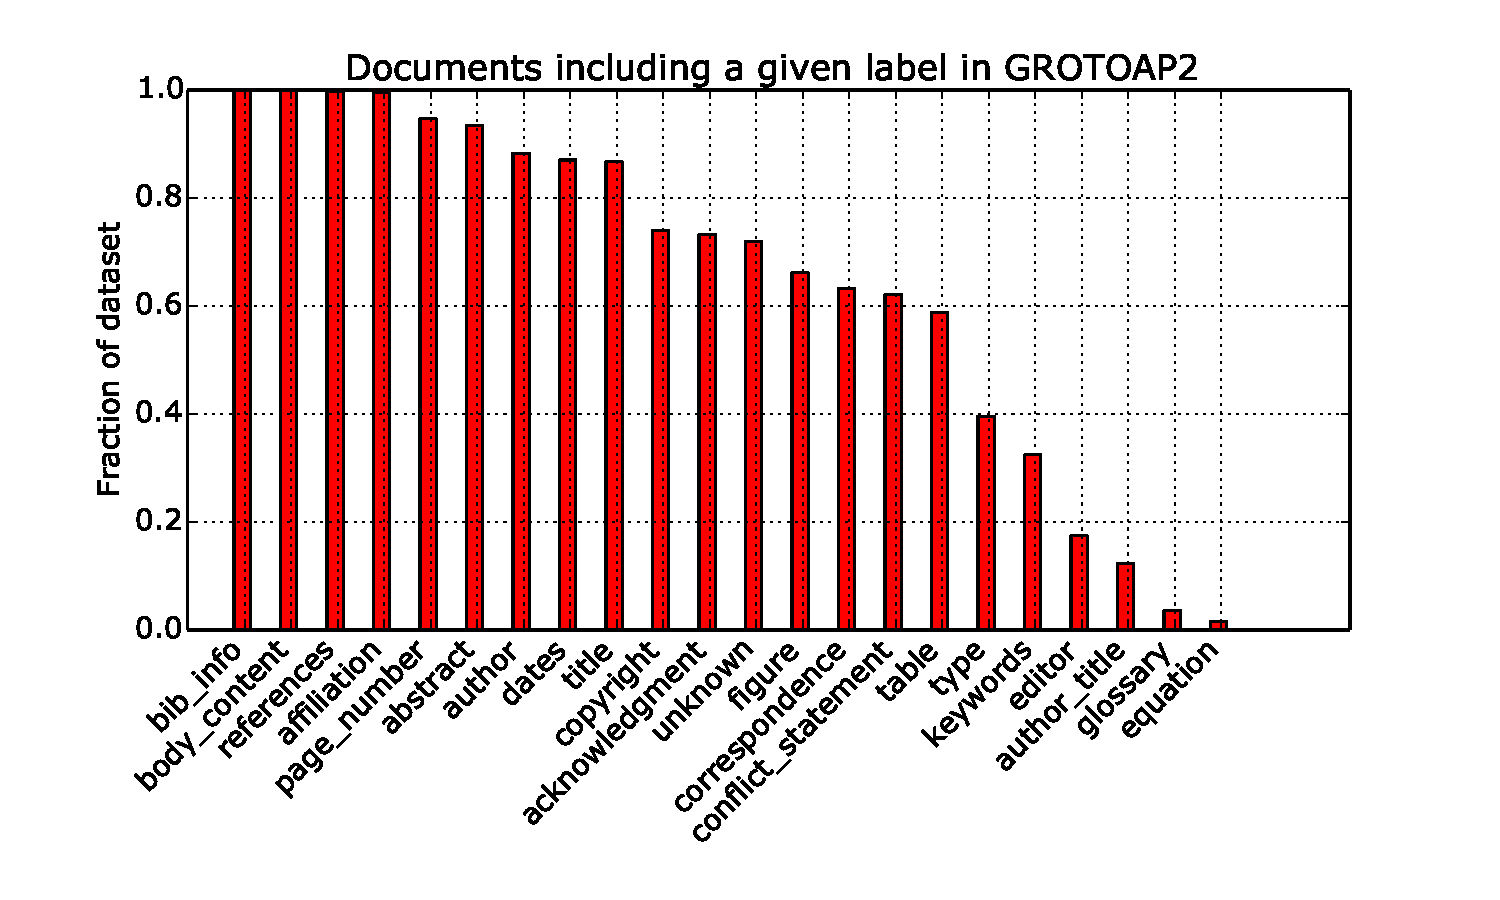
\includegraphics[width=18cm]{plots/docs_with_labels_barplot}}
  \caption{Barplot of fraction of documents containing given label}
  \label{fig:label_barplot}
\end{minipage}
\begin{minipage}[t!]{\linewidth}
  \centerline{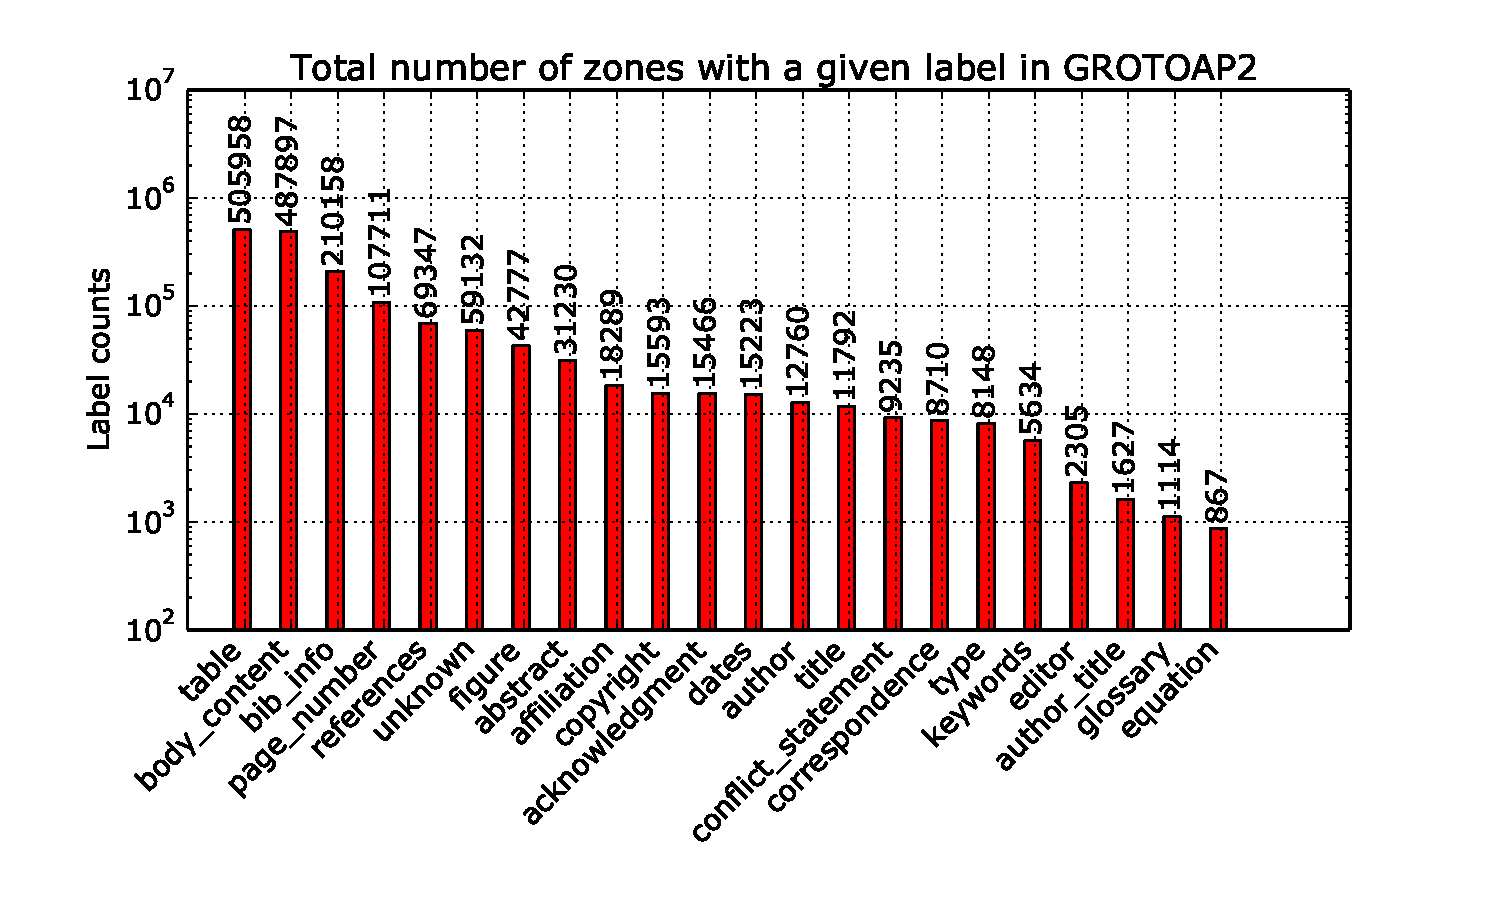
\includegraphics[width=18cm]{plots/label_barplot}}
  \caption{Barplot of total count of zones labeled with given label in GROTOAP2}
  \label{fig:label_count_barplot}
\end{minipage}
\end{figure}

  \begin{figure}
  \centering
\begin{minipage}[t!]{\linewidth}
  \centerline{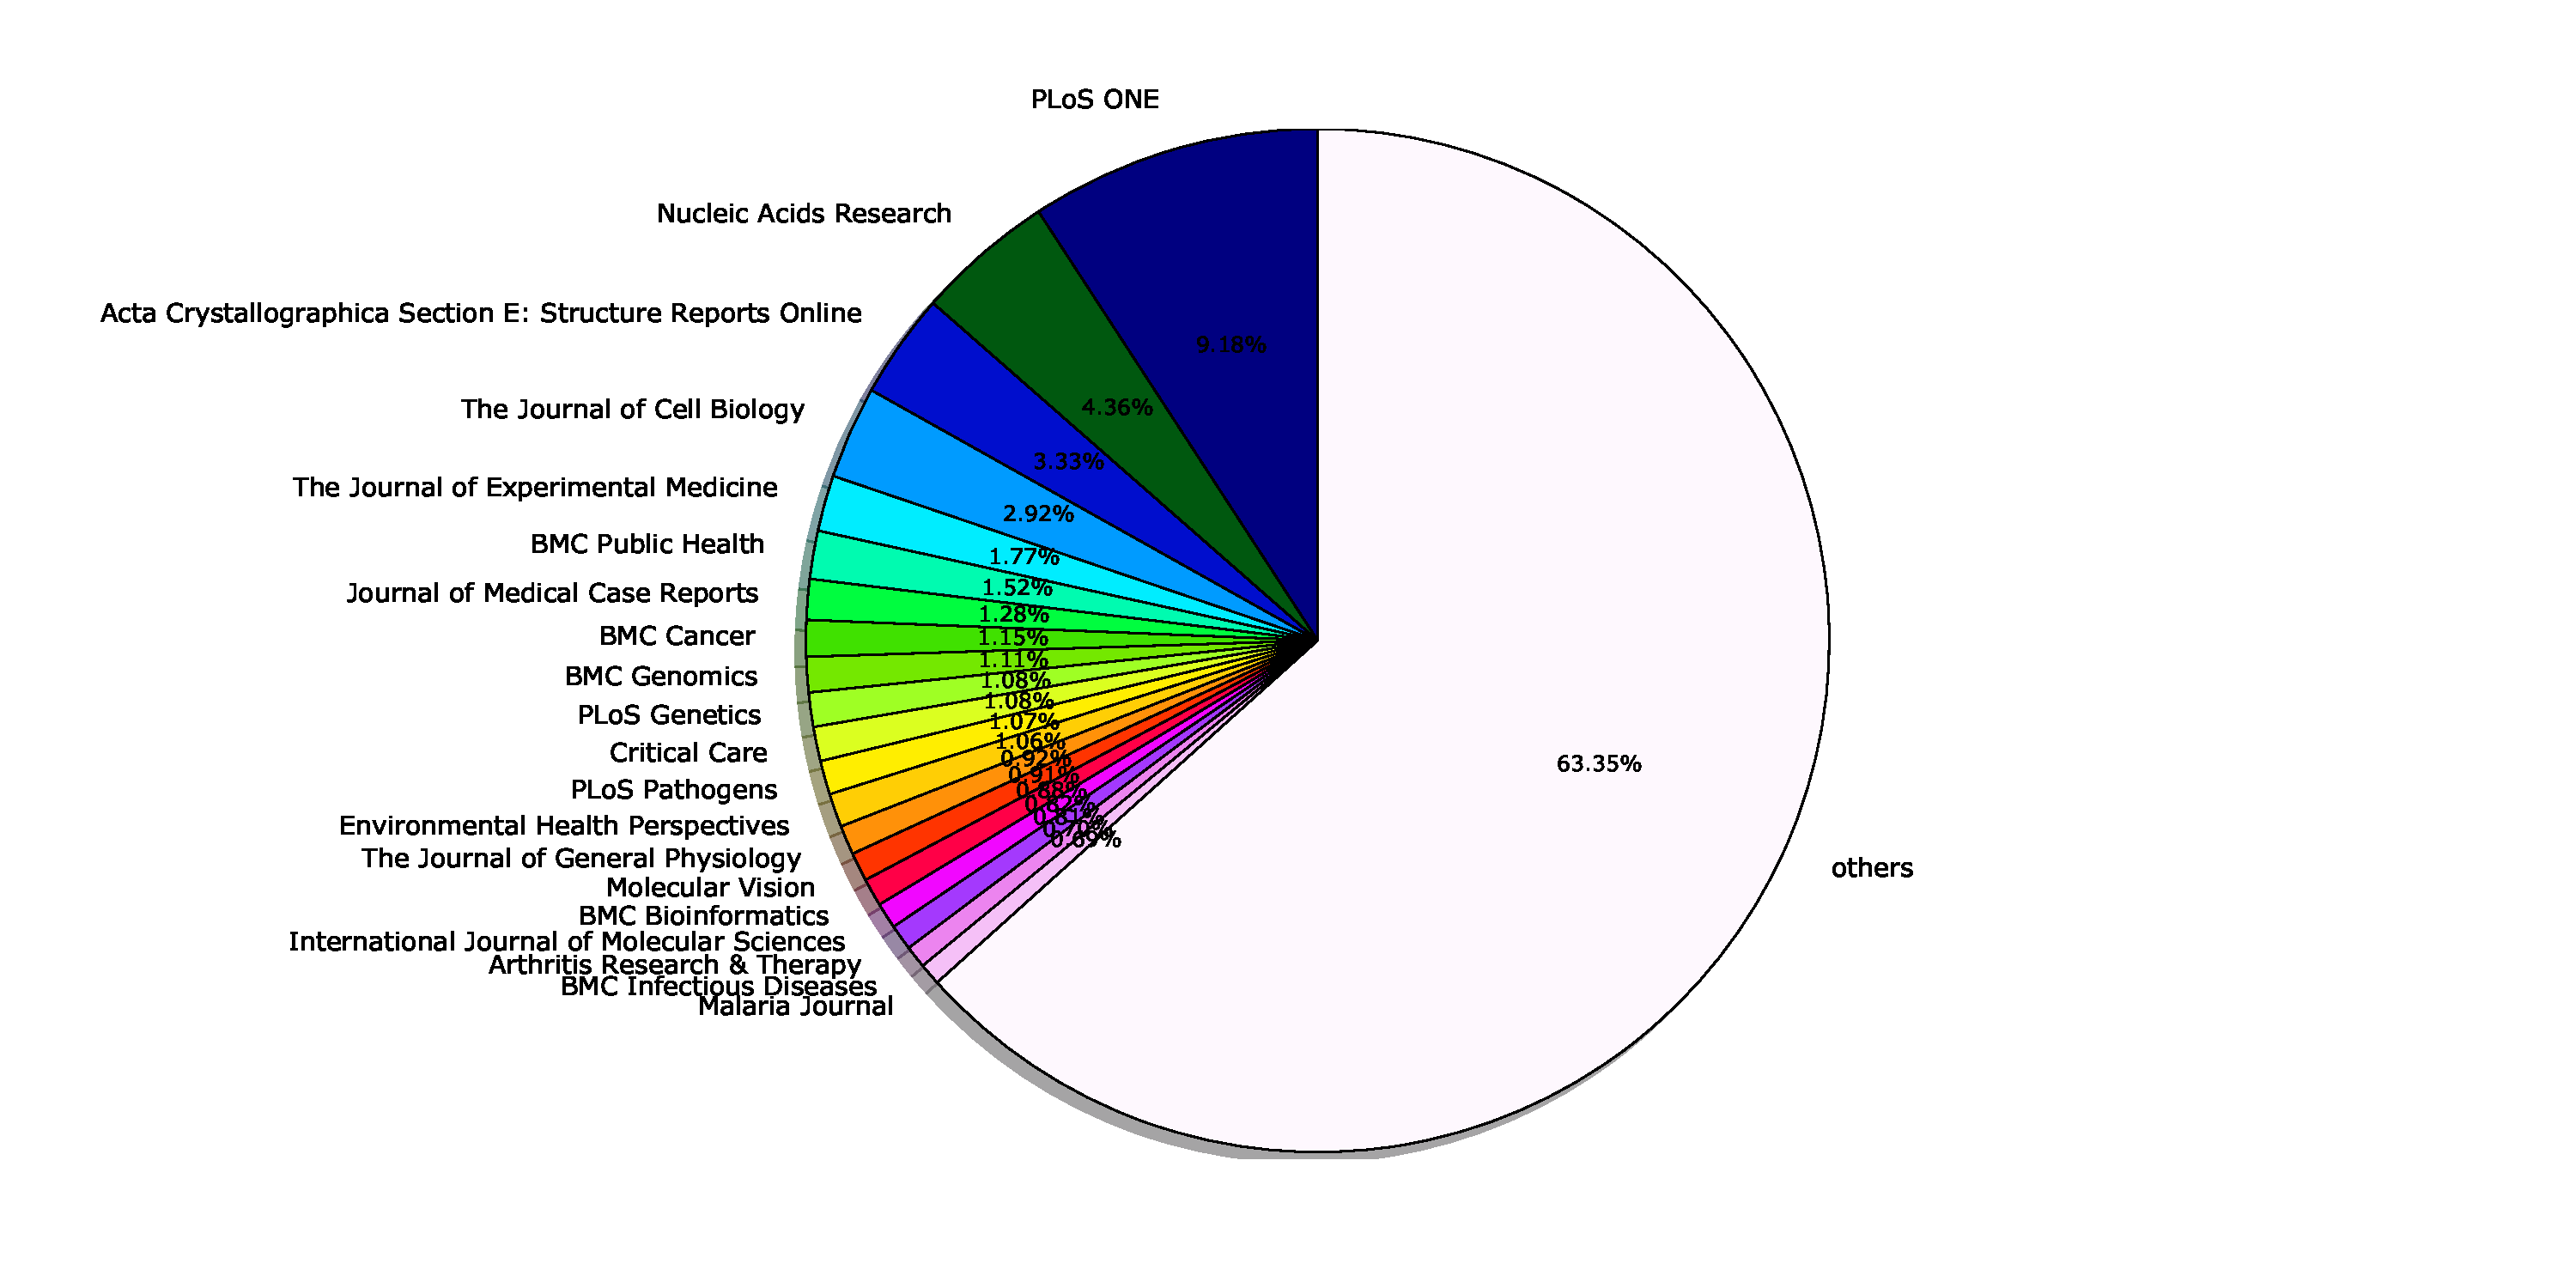
\includegraphics[width=22cm]{plots/journals_pieplot}}
  \caption{Top 25 journals in the GROTOAP2 dataset}
  \label{fig:journals_pieplot}
\end{minipage}
\quad
\begin{minipage}[t!]{\linewidth}
  \centerline{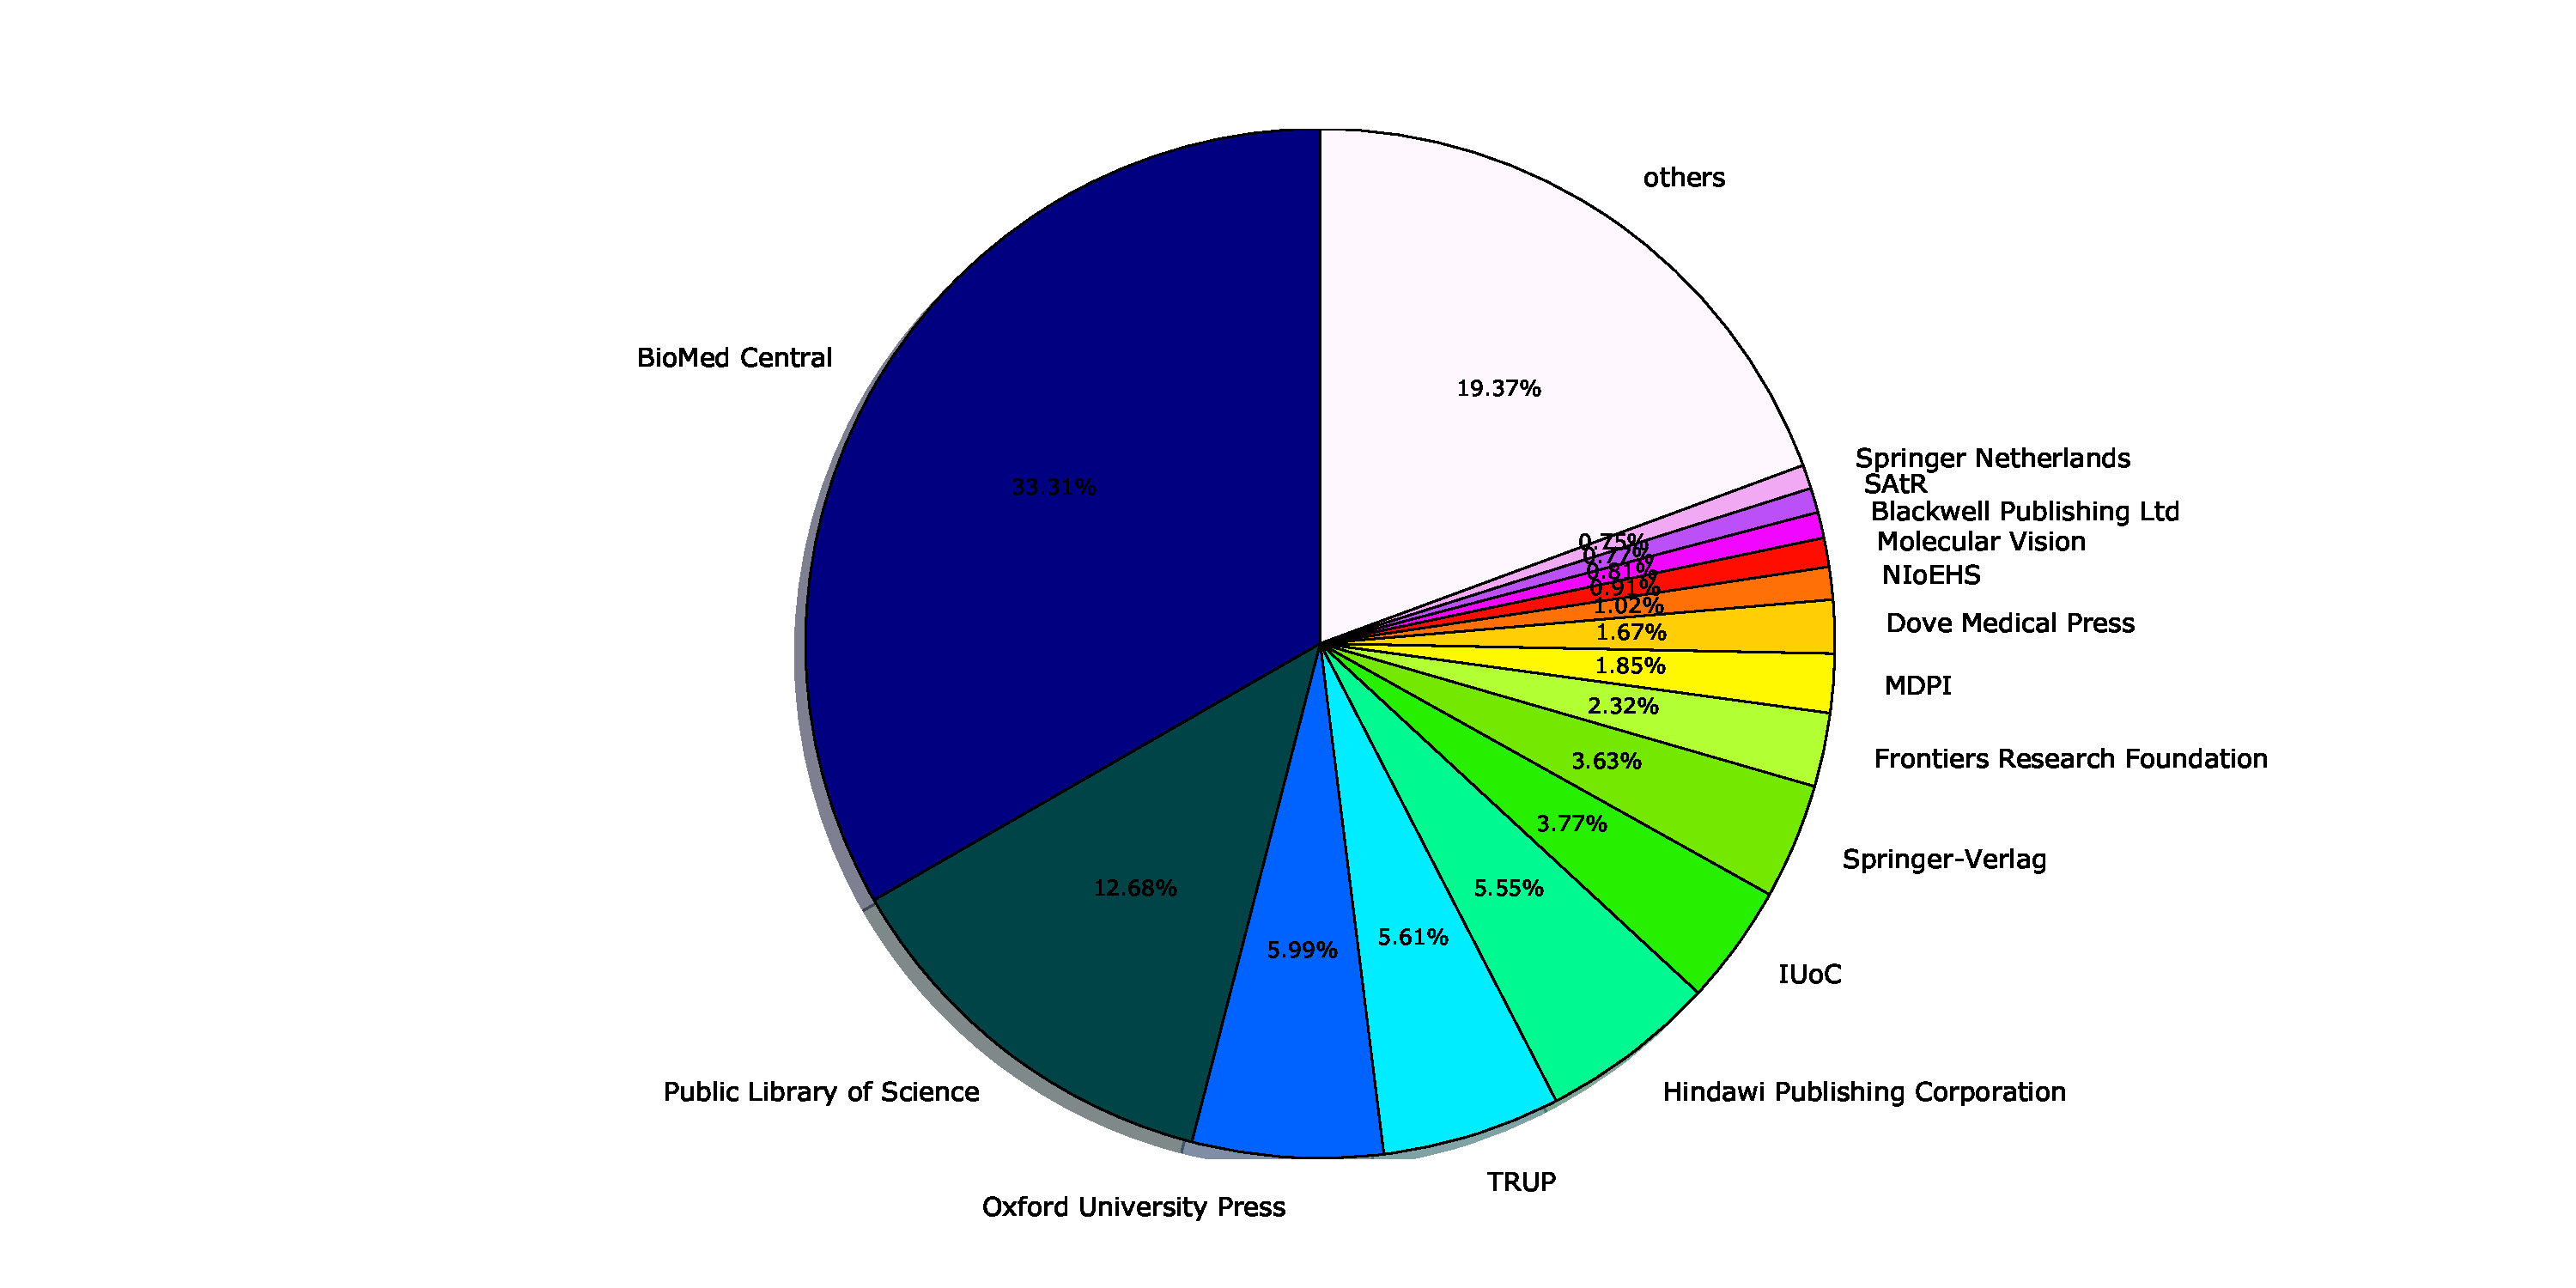
\includegraphics[width=22cm]{plots/publishers_pieplot}}
  \caption{Top 15 publishers in the GROTOAP2 dataset}
  \label{fig:publishers_pieplot}
\end{minipage}
\end{figure}
%%%%%%%%%%%%%%%%%%%%%%%%%%%%%%%%%%%%%%%%%%%

\begin{figure}
  \centering
\begin{minipage}[t!]{0.45\linewidth}
  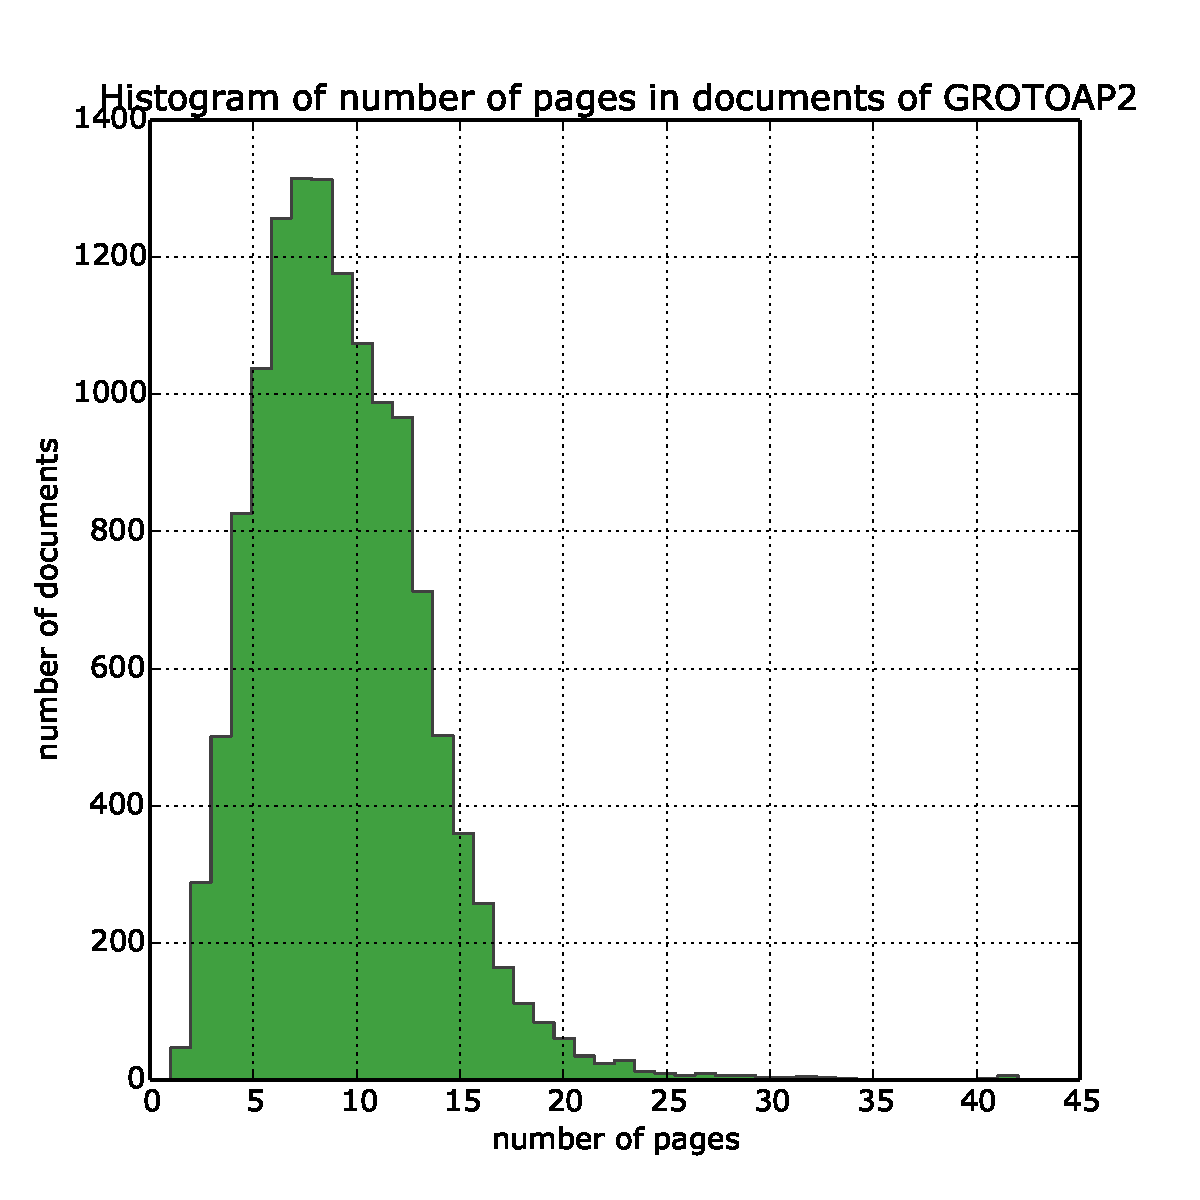
\includegraphics[width=8cm]{plots/pages_histogram}
  \caption{Histogram of number of pages of the documents in the GROTOAP2 dataset}
  \label{fig:page_count_histogram}
\end{minipage}
\quad
\begin{minipage}[t!]{0.45\linewidth}
  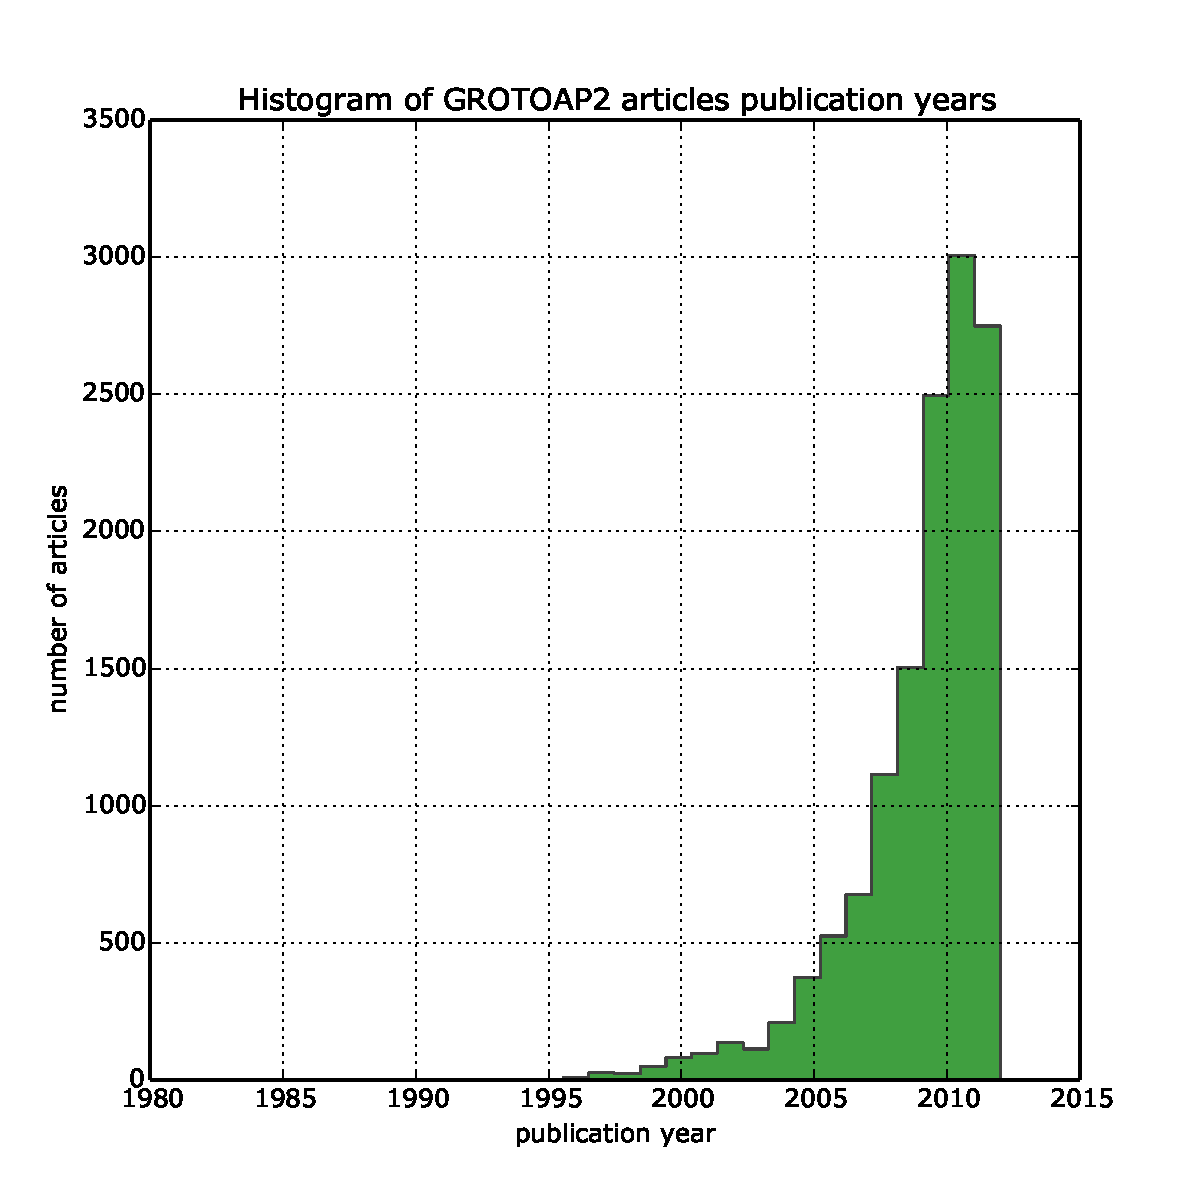
\includegraphics[width=8cm]{plots/publication_year_histogram}
  \caption{Histogram of publication year of the documents in the GROTOAP2 dataset}
  \label{fig:publication_year_histogram}
\end{minipage}
\end{figure}

\section{Dataset evaluation}
Evaluation of the created dataset is precisely described in \cite{DominikaTkaczykPaweSzostek2014}. Evaluation was not done by the author of this thesis. It was entirely performed by author's team mates from the Interdisciplinary Center for Mathematical and Computation Modeling. Nevertheless, its results and methodology will be quoted here in order to make the description more complete.

\quad
For the purpose of evaluation there was a handful of 50 documents picked. Those documents were automatically labeled and then errors were rectified. Subsequently, the corrected documents and the original ones were compared and the factors of precision and recall were calculated. Table \ref{tab:grotoap2_evaluation} shows the values obtained for each label.

\begin{table*}
%\ra{1.3}
\centering
\begin{tabular}{@{}rrrcrrr@{}}
 \toprule
label & precision & recall & \phantom{abc} & label & precision & recall\\ \midrule
abstract & 0.98 & 0.98 && equation & - & - \\ 
acknowledgment & 1.00 & 0.90 && figure & 0.99 & 0.46 \\ 
affiliation & 0.95 & 0.95 && glossary & 1.00 & 1.00 \\ 
author & 1.00 & 0.98 && keywords & 1.00 & 0.94 \\ 
author\_title & 1.00 & 1.00 && page\_number & 0.98 & 0.97 \\ 
bib\_info & 0.96 & 0.94 && references & 0.99 & 0.95 \\ 
body & 0.88 & 0.99 && table & 0.98 & 0.96 \\ 
conflict\_statement & 0.82 & 0.89 && title & 1.00 & 1.00 \\ 
copyright & 0.93 & 0.78 && type & 0.89 & 0.47 \\ 
correspondence & 1.00 & 0.97 && unknown & 0.62 & 0.94 \\ 
dates & 0.94 & 1.00 && * & 0.95 & 0.91 \\ 
editor & 1.00 & 1.00 &&   &      &       \\
\bottomrule
\end{tabular}
\caption{Evaluation metrics for the GROTOAP2 zone labeling process. The automatically generated metrics were manually compared with the actual labels on a subset of GROTOAP2. For each class precision and recall were calculated. Source: \cite{DominikaTkaczykPaweSzostek2014}}
\label{tab:grotoap2_evaluation}
\end{table*}

Another evaluation of the dataset was done by comparing CERMINE performance in two scenarios: trained with GROTOAP and a random handful of 1000 documents from GROTOAP2. Test documents were randomly selected from the Pubmed Central collection. Table \ref{tab:grotoap2_cermine_evaluation} shows results of the evaluation. One can notice that the F-score of classifier based on GROTOAP2 has grown by 16.93\%.

\begin{table*}[]
\centering
\begin{tabular}{@{}rrr@{}}
\toprule
& GROTOAP & GROTOAP2 \\
\midrule
precision & 77.13\% & 82.22\% \\
recall & 55.99\% & 76.96\% \\
F-score & 62.41\% & 79.34\% \\
\bottomrule
\end{tabular}
\caption{Evaluation of GROTOAP2 using CERMINE trained with GROTOAP and GROTOAP2.}
\label{tab:grotoap2_cermine_evaluation}
\end{table*}


\include{results}
\begin{appendices}
%\appendixpage
\noappendicestocpagenum
\addappheadtotoc

\chapter{Description of classification features}
\label{appendix:features}
\newgeometry{left=2cm,right=2cm}
%\begin{landscape}

\begin{longtable}[t!]{l|l|p{9cm}}
\hline
\# & \textbf{Feature Name} & \textbf{Description} \\ \hline
\rownumber & AffiliationFeature & Tells if the zone contains one of the \{``author details'', ``university'', ``department'', ``school'', ``institute'', ``affiliation''\}\\ \hline
\rownumber & AuthorFeature & Tells if a text zone contains a word starting with ``author''\\ \hline
\rownumber & BibinfoFeature & Number of occurences of \{``cite'', ``pages'', ``article'', ``volume'', ``publishing'', ``journal'', ``doi'', ``cite this article'', ``citation'', ``issue'', ``issn''\} \\ \hline
\rownumber & BracketRelativeCount & Ratio of the number of brackets to the number of all characters \\ \hline
\rownumber & BracketedLineRelativeCount & Ratio of number of lines starting with a bracket to the number of all lines\\ \hline
\rownumber & CharCountFeature & Counts number of characters in a zone\\ \hline
\rownumber & CharCountRelativeFeature & Ratio of number of characters in a zone to the number of character on its page\\ \hline
\rownumber & CommaCountFeature & Counts number of commas in a zone\\ \hline
\rownumber & CommaRelativeCountFeature & Ratio of commas to all characters in a zone \\ \hline
\rownumber & ContainsPageNumberFeature & Tells consists of a number or is like ``Page \%d'' or ``page \%d'', where \%d is a number \\ \hline
\rownumber & CuePhrasesRelativeCountFeature & Ratio of cue phrases from \{``although'', ``therefore'', ``therein'', ``hereby'', ``nevertheless'', ``to this end'', ``however'', ``moreover'', ``nonetheles''\} to all words\\ \hline
\rownumber & DateFeature & Tells if the zone contains a string being a date with months expressed as text or as a number, with either European or American order\\ \hline
\rownumber & DigitCountFeature & Number of digits is in the zone\\ \hline
\rownumber & DigitRelativeCountFeature & Ratio of digits to all characters in the zone \\ \hline
\rownumber & DistanceFromNearestNeighbourFeature & Distance to the nearest neighbour zone or returns Double.MAX\_VALUE if there is no other zone on the page\\ \hline
\rownumber & DotCountFeature & Counts number of dots (``.'') in the zone\\ \hline
\rownumber & DotRelativeCountFeature & Ratio of number of dots to all characters in the zone \\ \hline
\rownumber & EmailFeature & Tells if the zone contains a valid e-mail address\\ \hline
\rownumber & EmptySpaceRelativeFeature & Calculates a ratio of the surface taken by the characters' bounding boxes to the area of the zone \\ \hline
\rownumber & FontHeightMeanFeature & Calculates average font size in the zone \\ \hline
\rownumber & FreeSpaceWithinZoneFeature & Difference between zone's area and total area taken by the characters\\ \hline
\rownumber & HeightFeature & Height of a zone\\ \hline
\rownumber & HeightRelativeFeature & Ratio of zone's height to the page's height\\ \hline
\rownumber & HorizontalRelativeProminenceFeature & Area taken by the zone and free area to the West and East of the page. This features tries to fit into the page a bounding box of the same height as the zone and sticking either to neighbour zones or to the page boundaries in E and W\\ \hline
\rownumber & IsAnywhereElseFeature & Tells if this zone is duplicated anywhere in the investigated document \\ \hline
\rownumber & IsFirstPageFeature & Tells if the zone is located on the first page of the document \\ \hline
\rownumber & IsFontBiggerThanNeighboursFeature & Tells whether the font of the zone is bigger than in neighbour zones\\ \hline
\rownumber & IsGreatestFontOnPageFeature & Tells if the zone has the greatest font on the page \\ \hline
\rownumber & IsHighestOnThePageFeature & Tells if the zone is the highest on the page \\ \hline
\rownumber & IsItemizeFeature & Tells if the zone contains any kind of indexing charactersic for section or enumeration numbering \\ \hline
\rownumber & IsWidestOnThePageFeature & Tells if the zone is the widest on the page\\ \hline
\rownumber & IsLastButOnePageFeature & Tells if the zone is located on the last but one page\\ \hline
\rownumber & IsLastPageFeature & Tells if the zone is located on the last page\\ \hline
\rownumber & IsLeftFeature & Tells if the zone is in the left part of the page\\ \hline
\rownumber & IsLongestOnThePageFeature & Tells if the zone contains maximal number of characters among all the zones in the page\\ \hline
\rownumber & IsLowestOnThePageFeature & Tells if the zone is most southern on the page (southern bounding box border is taken into account) \\ \hline
\rownumber & IsOnSurroundingPagesFeature & Tells if the same zone is on the previous or on the next page \\ \hline
\rownumber & IsPageNumberFeature & Tells if a zone is entirely a number \\ \hline
\rownumber & IsRightFeature & Tells if a zone is on the east side of the page\\ \hline
\rownumber & IsSingleWordFeature & Tells if a zone is one word \\ \hline
\rownumber & LastButOneZoneFeature & Tells if the zone is last but one wrt. to the reading order \\ \hline
\rownumber & LineCountFeature & Number of lines in the zone\\ \hline
\rownumber & LineRelativeCountFeature & Ratio of lines in the to all lines on the page\\ \hline
\rownumber & LineHeightMeanFeature & Mean height of the zone\\ \hline
\rownumber & LineWidthMeanFeature & Mean width of the zone's lines\\ \hline
\rownumber & LineXPositionMeanFeature & Mean distance of zone's lines to the zone's bounding box \\ \hline
\rownumber & LineXPositionDiffFeature & The feature looks at the left border of all lines within a zone and finds the most-eastern and most-western among them. A positive difference between these two values is returned\\ \hline
\rownumber & LineXWidthPositionDiffFeature & Difference between mean value of lines' left border X coordinate and zone's  \\ \hline
\rownumber & LetterCountFeature & Number of letters in the zone\\ \hline
\rownumber & LetterRelativeCountFeature & Ratio of letters in the zone to all letters on the page\\ \hline
\rownumber & LowercaseCountFeature & Number of letters in lower case in the zone\\ \hline
\rownumber & LowercaseRelativeCountFeature & Number of letters in lower case in the zone\\ \hline
\rownumber & PageNumberFeature & Page number wrt. the reading order \\ \hline
\rownumber & PreviousZoneFeature & Value of label assigned to the previous zone wrt. the reading order\\ \hline
\rownumber & ProportionsFeature & Width to height ratio\\ \hline
\rownumber & PunctuationRelativeCountFeature & Ratio of punctuation marks to all characters in the zone\\ \hline
\rownumber & ReferencesFeature & Number of characteristic enumeration indices in the zone, e.g. ``1.''.\\ \hline
\rownumber & StartsWithDigitFeature & Tells if the zone's first character is a digit\\ \hline
\rownumber & UppercaseCountFeature & Number of upper case characters in the zone \\ \hline
\rownumber & UppercaseRelativeCountFeature & Ratio of upper case letters to all characters\\ \hline
\rownumber & UppercaseWordCountFeature & Number of words starting with upper case\\ \hline
\rownumber & UppercaseWordRelativeCountFeature & Ratio of upper case words to all words\\ \hline
\rownumber & VerticalProminenceFeature & Space taken by the zone and free area to the North and South of the page. This features tries to fit into the page a bounding box of the same height as the zone and sticking either to neighbour zones or to the page boundaries in N and S \\ \hline
\rownumber & WidthFeature & Width of the bounding box in pixels\\ \hline
\rownumber & WordCountFeature & Number of words in the zone\\ \hline
\rownumber & WordCountRelativeFeature & Ratio of number of words in the zone to all words in the page\\ \hline
\rownumber & WordWidthMeanFeature & Mean width of words in the zone expressed as pixels\\ \hline
\rownumber & WordLengthMeanFeature & Mean width of words in the zone expressed as number of characters\\ \hline
\rownumber & WordLengthMedianFeature & Median of number of characters in all words \\ \hline
\rownumber & WhitespaceCountFeature & Number of white characters in the text\\ \hline
\rownumber & WhitespaceRelativeCountLogFeature & Feature calculated as $-log \frac{S}{L}$ where $S$ is zone's empty area and $L$ is zone's text length \\ \hline
\rownumber & WidthRelativeFeature & Ratio of zone's width to page's width\\ \hline
\rownumber & XPositionFeature & X coordinate\\ \hline
\rownumber & XPositionRelativeFeature & Ratio of zone's X coordinate to page's width \\ \hline
\rownumber & YPositionFeature & Y coordinate \\ \hline
\rownumber & YPositionRelativeFeature & Ratio of zone's Y coordinate to page's height \\ \hline
\end{longtable}
\restoregeometry
\setcounter{magicrownumbers}{0}
\end{appendices}
%\addtocontents{toc}{\protect\vspace{1em}\noindent{\bf Bibliografia}\hspace*{\fill}{\bf \pageref{literatura}}}
\pagebreak
\nocite{*}
\bibliography{bibliography}{}
\bibliographystyle{plain}
\end{document}

